% Options for packages loaded elsewhere
\PassOptionsToPackage{unicode}{hyperref}
\PassOptionsToPackage{hyphens}{url}
%
\documentclass[
  12pt,
  man, donotrepeattitle,floatsintext]{apa6}
\usepackage{amsmath,amssymb}
\usepackage{iftex}
\ifPDFTeX
  \usepackage[T1]{fontenc}
  \usepackage[utf8]{inputenc}
  \usepackage{textcomp} % provide euro and other symbols
\else % if luatex or xetex
  \usepackage{unicode-math} % this also loads fontspec
  \defaultfontfeatures{Scale=MatchLowercase}
  \defaultfontfeatures[\rmfamily]{Ligatures=TeX,Scale=1}
\fi
\usepackage{lmodern}
\ifPDFTeX\else
  % xetex/luatex font selection
  \setmainfont[]{Times New Roman}
\fi
% Use upquote if available, for straight quotes in verbatim environments
\IfFileExists{upquote.sty}{\usepackage{upquote}}{}
\IfFileExists{microtype.sty}{% use microtype if available
  \usepackage[]{microtype}
  \UseMicrotypeSet[protrusion]{basicmath} % disable protrusion for tt fonts
}{}
\makeatletter
\@ifundefined{KOMAClassName}{% if non-KOMA class
  \IfFileExists{parskip.sty}{%
    \usepackage{parskip}
  }{% else
    \setlength{\parindent}{0pt}
    \setlength{\parskip}{6pt plus 2pt minus 1pt}}
}{% if KOMA class
  \KOMAoptions{parskip=half}}
\makeatother
\usepackage{xcolor}
\usepackage{graphicx}
\makeatletter
\def\maxwidth{\ifdim\Gin@nat@width>\linewidth\linewidth\else\Gin@nat@width\fi}
\def\maxheight{\ifdim\Gin@nat@height>\textheight\textheight\else\Gin@nat@height\fi}
\makeatother
% Scale images if necessary, so that they will not overflow the page
% margins by default, and it is still possible to overwrite the defaults
% using explicit options in \includegraphics[width, height, ...]{}
\setkeys{Gin}{width=\maxwidth,height=\maxheight,keepaspectratio}
% Set default figure placement to htbp
\makeatletter
\def\fps@figure{htbp}
\makeatother
\setlength{\emergencystretch}{3em} % prevent overfull lines
\providecommand{\tightlist}{%
  \setlength{\itemsep}{0pt}\setlength{\parskip}{0pt}}
\setcounter{secnumdepth}{-\maxdimen} % remove section numbering
% Make \paragraph and \subparagraph free-standing
\ifx\paragraph\undefined\else
  \let\oldparagraph\paragraph
  \renewcommand{\paragraph}[1]{\oldparagraph{#1}\mbox{}}
\fi
\ifx\subparagraph\undefined\else
  \let\oldsubparagraph\subparagraph
  \renewcommand{\subparagraph}[1]{\oldsubparagraph{#1}\mbox{}}
\fi
\newlength{\cslhangindent}
\setlength{\cslhangindent}{1.5em}
\newlength{\csllabelwidth}
\setlength{\csllabelwidth}{3em}
\newlength{\cslentryspacingunit} % times entry-spacing
\setlength{\cslentryspacingunit}{\parskip}
\newenvironment{CSLReferences}[2] % #1 hanging-ident, #2 entry spacing
 {% don't indent paragraphs
  \setlength{\parindent}{0pt}
  % turn on hanging indent if param 1 is 1
  \ifodd #1
  \let\oldpar\par
  \def\par{\hangindent=\cslhangindent\oldpar}
  \fi
  % set entry spacing
  \setlength{\parskip}{#2\cslentryspacingunit}
 }%
 {}
\usepackage{calc}
\newcommand{\CSLBlock}[1]{#1\hfill\break}
\newcommand{\CSLLeftMargin}[1]{\parbox[t]{\csllabelwidth}{#1}}
\newcommand{\CSLRightInline}[1]{\parbox[t]{\linewidth - \csllabelwidth}{#1}\break}
\newcommand{\CSLIndent}[1]{\hspace{\cslhangindent}#1}
\ifLuaTeX
\usepackage[bidi=basic]{babel}
\else
\usepackage[bidi=default]{babel}
\fi
\babelprovide[main,import]{english}
\ifPDFTeX
\else
\babelfont{rm}[]{Times New Roman}
\fi
% get rid of language-specific shorthands (see #6817):
\let\LanguageShortHands\languageshorthands
\def\languageshorthands#1{}
% Manuscript styling
\usepackage{upgreek}
\captionsetup{font=singlespacing,justification=justified}

% Table formatting
\usepackage{longtable}
\usepackage{lscape}
% \usepackage[counterclockwise]{rotating}   % Landscape page setup for large tables
\usepackage{multirow}		% Table styling
\usepackage{tabularx}		% Control Column width
\usepackage[flushleft]{threeparttable}	% Allows for three part tables with a specified notes section
\usepackage{threeparttablex}            % Lets threeparttable work with longtable

% Create new environments so endfloat can handle them
% \newenvironment{ltable}
%   {\begin{landscape}\centering\begin{threeparttable}}
%   {\end{threeparttable}\end{landscape}}
\newenvironment{lltable}{\begin{landscape}\centering\begin{ThreePartTable}}{\end{ThreePartTable}\end{landscape}}

% Enables adjusting longtable caption width to table width
% Solution found at http://golatex.de/longtable-mit-caption-so-breit-wie-die-tabelle-t15767.html
\makeatletter
\newcommand\LastLTentrywidth{1em}
\newlength\longtablewidth
\setlength{\longtablewidth}{1in}
\newcommand{\getlongtablewidth}{\begingroup \ifcsname LT@\roman{LT@tables}\endcsname \global\longtablewidth=0pt \renewcommand{\LT@entry}[2]{\global\advance\longtablewidth by ##2\relax\gdef\LastLTentrywidth{##2}}\@nameuse{LT@\roman{LT@tables}} \fi \endgroup}

% \setlength{\parindent}{0.5in}
% \setlength{\parskip}{0pt plus 0pt minus 0pt}

% Overwrite redefinition of paragraph and subparagraph by the default LaTeX template
% See https://github.com/crsh/papaja/issues/292
\makeatletter
\renewcommand{\paragraph}{\@startsection{paragraph}{4}{\parindent}%
  {0\baselineskip \@plus 0.2ex \@minus 0.2ex}%
  {-1em}%
  {\normalfont\normalsize\bfseries\itshape\typesectitle}}

\renewcommand{\subparagraph}[1]{\@startsection{subparagraph}{5}{1em}%
  {0\baselineskip \@plus 0.2ex \@minus 0.2ex}%
  {-\z@\relax}%
  {\normalfont\normalsize\itshape\hspace{\parindent}{#1}\textit{\addperi}}{\relax}}
\makeatother

\makeatletter
\usepackage{etoolbox}
\patchcmd{\maketitle}
  {\section{\normalfont\normalsize\abstractname}}
  {\section*{\normalfont\normalsize\abstractname}}
  {}{\typeout{Failed to patch abstract.}}
\patchcmd{\maketitle}
  {\section{\protect\normalfont{\@title}}}
  {\section*{\protect\normalfont{\@title}}}
  {}{\typeout{Failed to patch title.}}
\makeatother

\usepackage{xpatch}
\makeatletter
\xapptocmd\appendix
  {\xapptocmd\section
    {\addcontentsline{toc}{section}{\appendixname\ifoneappendix\else~\theappendix\fi\\: #1}}
    {}{\InnerPatchFailed}%
  }
{}{\PatchFailed}
\keywords{bibliometrics, collaboration, colonialism, Global South, scholarly societies, scientometrics, temperate, text-mining}
\usepackage{lineno}

\linenumbers
\usepackage{csquotes}
\usepackage{fancyhdr}
\pagestyle{empty}
\pagestyle{fancy}
\fancyfoot[C]{\thepage}
\fancyhead[L]{Bruna}
\fancyhead[R]{ATBC Presidential Plenary}
\usepackage{float}
\floatplacement{figure}{H}
\usepackage{booktabs}
\usepackage{setspace}
\raggedbottom
\usepackage{tabu}
\usepackage{makecell}
\usepackage{pdflscape}
\usepackage{longtable}
\newcommand{\blandscape}{\begin{landscape}}
\newcommand{\elandscape}{\end{landscape}}
\usepackage{parskip}
\setlength{\parskip}{0pt}
\setlength\parindent{22pt}
\ifLuaTeX
  \usepackage{selnolig}  % disable illegal ligatures
\fi
\IfFileExists{bookmark.sty}{\usepackage{bookmark}}{\usepackage{hyperref}}
\IfFileExists{xurl.sty}{\usepackage{xurl}}{} % add URL line breaks if available
\urlstyle{same}
\hypersetup{
  pdfauthor={Emilio M. Bruna1, 2, 3},
  pdflang={en-EN},
  pdfkeywords={bibliometrics, collaboration, colonialism, Global South, scholarly societies, scientometrics, temperate, text-mining},
  hidelinks,
  pdfcreator={LaTeX via pandoc}}

\title{\flushleft \textbf{Is there really such a thing as \textit{Tropical} Biology?}\footnote{Inspired by the provocative title of M. H. Robinson's 1978 essay in the journal \emph{Tropical Ecology}.}}
\author{Emilio M. Bruna\textsuperscript{1, 2, 3}}
\date{}


\shorttitle{LRH and RRH: Bruna}

\affiliation{\vspace{0.5cm}\textsuperscript{1} Department of Wildlife Ecology and Conservation, University of Florida, PO Box 110430, Gainesville, FL 32611-0430, USA\\\textsuperscript{2} Center for Latin American Studies, University of Florida, PO Box 115530, Gainesville, FL 32611-5530, USA\\\textsuperscript{3} Corresponding Author; email: \href{mailto:embruna@ufl.edu}{\nolinkurl{embruna@ufl.edu}}}

\note{

\thispagestyle{otherpage}

\vspace{7cm}

\flushleft Received:\_\_\_\_\_\_; Revised:\_\_\_\_\_\_; Accepted:\_\_\_\_\_\_.

}

\abstract{%
The ecosystems of The Tropics comprise the majority of the planet's biodiversity, approximately 40\% of its terrestrial surface area, and half the human population. Depsite this, Tropical Biology has historically been conceptualized as a specialized subdiscipline of the Biological Sciences. I assessed the validity of this assumption, and conclude that the answer depends on the evidence and logic used to evaluate it. I suggest that the way forward as a discipline is not for Tropical Biologists to drop the adjective that unites them, but to recenter The Tropics as the the foundational ecosystems of ecology and evolutionary biology.
}



\begin{document}
\maketitle

\onehalfspacing

\doublespacing

\hypertarget{introduction}{%
\subsection{1. INTRODUCTION}\label{introduction}}

\noindent \emph{``This is an interesting and useful study, but I feel the manuscript is better suited to a specialized journal focusing on tropical ecosystems.''}

\hfill Subject Editor \emph{(name and journal redacted)}

\bigskip

\noindent This decision regarding my submission to one of our field's well-known journals is likely familiar to many members of the Association for Tropical Biology \& Conservation (ATBC). All three reviews were positive, with none of the referees identifying significant shortcomings or requesting major changes. So why had the manuscript been rejected? My only clue was in the Editor's conclusion, from which I gathered they felt studies done \emph{in} the tropics were of limited relevance to researchers working \emph{outside} the tropics. That's for whom a specialized journal is published, after all -- a smaller community of subject-matter experts -- and the journal to which we had submitted our study sought to publish ``broad conceptual advances''. In short, the Subject Editor was drawing a distinction between Biology and \emph{Tropical} Biology, with the latter a specialized subdiscipline of the former.\\
This provincial view of research done in the tropics is not new. In 1963, P. W. Richards felt it necessary to use his Presidential Address to the British Ecological Society to explain ``what the Tropics can contribute to ecology'', advocate for financial investment in tropical research and field stations, and encourage students to visit and dedicate study ``the most {[}biologically{]} exciting part of the world'' (Richards 1963). His justification for this topic was self-deprecating but pointed --- he was concerned that a talk summarizing recent advances in tropical ecology ``would probably bore the large part of my audience who have never been to the tropics and never intend to do so'' (Richards 1963). That he felt this advocacy was necessary despite decades of effort (Richards 1946, 1964) must have been extremely frustrating.

Sixty years on many of us find ourselves similarly frustrated. Field stations in the tropics remain underfunded (Chapman \emph{et al.} 1945, Corner 1946, Eppley \emph{et al.} 2024). Financial support for tropical research continues to decline (Chapman \emph{et al.} 1945, Sohmer 1980, Stegmann \emph{et al.} 2024). And despite tropical ecosystems comprising the majority of the planet's biodiversity (Gaston 2000), approximately 40\% of its terrestrial surface area, and half the human population (Hoornweg \& Pope 2017), their study continues to be seen by many as a scientific specialization. My objective here is not to review the biological validity (Robinson 1978, Moles \& Ollerton 2016) or scientific implications (Zuk 2016) of this generalization, nor to summarize the history, status, and direction of tropical research (\emph{e.g.,} Buechner \& Fosberg 1967, Janzen 1972, Janzen 1986, Chazdon \& Whitmore 2001, Bawa \emph{et al.} 2004). Instead, I will attempt to assess the fundamental assumption behind the Editor's summary that motivated this essay: Is there really such a thing as \emph{Tropical} Biology?

\hypertarget{why-the-answer-is-no.}{%
\subsection{\texorpdfstring{1. Why the answer is \emph{`No'.}}{1. Why the answer is `No'.}}\label{why-the-answer-is-no.}}

\noindent \emph{``\ldots in the case of biology, a major part of the accumulated biological knowledge is concerned with a rather minor part of the world's fauna and flora, because of the chance development of biology in the temperate zones.''}

\hfill S. D. Ripley (1967)
\bigskip

\noindent One means of assessing if \emph{Tropical} Biology is a distinct academic discipline is by considering the communities into which scientists self-organize. Scholarly societies are one such community; their establishment requires both an intellectual pursuit with which individuals identify and a critical mass of like-minded individuals in search of community. Some of these communities coalesce around broad conceptual domains (e.g., \emph{Evolutionary} Biology, \emph{Conservation} Biology, \emph{Integrative} Biology; Figure \ref{fig:fig-org}A). Still others bring together individuals from different conceptual domains that share an interest in a particular system (e.g., \emph{Avian} Biology, \emph{Island} Biology; Figure \ref{fig:fig-org}B). Finally, some scholarly societies comprise individuals grounded in a common methodological framework, though they may do so with disparate study systems or to address questions in distinct conceptual domains (e.g., \emph{Molecular} Biology, \emph{Mathematical} Biology, \emph{Systematic} Biology; Figure \ref{fig:fig-org}C).\\
\emph{Tropical} Biology fails to align with any of these constructs. Its practitioners investigate fundamental questions across conceptual domains with a broad range of methodological approaches and study systems. Put another way, ``The work that tropical biologists do is nearly as diverse as the ecosystems they study'' (Raby (2017a); p.~5). Moreover, the ``geographic pigeonhole'' (Raby 2017a) that would seem to unite this community of scientists --- the adjective `tropical' --- is itself difficult to operationalize. Formally, \emph{The Tropics} are the band of the Earth's surface receiving at least one day of direct overhead sunlight per year; this region is delineated by the Tropics of Capricorn and Cancer (23°26'10.4'' S and N, respectively). However, the ranges of many `tropical' species and ecosystems extend far beyond these boundaries\footnote{Perhaps the most extreme examples are migratory birds such as the northern wheatear (\emph{Oenanthe oenanthe}), which fly over 14,000 km from sub-Saharan Africa to their breeding grounds in the Arctic (Bairlein \emph{et al.} 2012)}, however, which is in part why feeleyWhereEarthAre2018 identified no less than eight distinct criteria by which authors to define `tropical' systems. How then is it that \emph{Tropical} Biology came to be seen as a distinct subdicipline, despite the lack the sharp boundaries around which scientific groups typically coalesce?

These contemporary perceptions of `The Tropics' as distant and different are the result of centuries of historical and cultural reinforcement (Arnold 1996, Driver \& Yeoh 2000, Stepan 2001, Miller \& Reill 2011). The first Europeans to visit the tropics returned with vivid, captivating, and frequently pejorative descriptions of the places and people they encountered (Putz \& Holbrook 1988). Their stories and images established a series of persistent, often contradictory tropes about tropical regions and people that were repeated and reinterpreted by subsequent visitors and inculcated by colonial expansion (Smith 1950, Stepan 2001). The historian David Arnold has argued that these narratives of \emph{Tropicality} (\emph{sensu} Gourou 1947), or even referring to this part of the globe as \emph{The Tropics}, allowed Europeans simultaneously define the region as environmentally and culturally distinct while also superimposing a common identity on very distinct parts of the tropical world (Arnold 1996).

The narratives of naturalists such as von Humboldt, Darwin, and Wallace were both informed by and reinforced these conceptions of the tropics as `distant' and `other' (Raby 2017a); their writing inspired many of the scientists central to the coalescing sciences of ecology and evolutionary biology. Another historian, Megan Raby, has elegantly demonstrated how the resulting scientific narratives, including the unique status of \emph{Tropical} Biology, were not simply distillations of prevailing cultural tropes. Instead they emerged from the complex interplay of the European colonialism, the expansion of US hegemony in Latin America and the Caribbean at the turn of the twentieth century, and the establishment of new field stations as tropical outposts for North American scientists that accompanied this political and economic expansion (Raby 2017a). The role of this scientific colonialism at such a pivotal moment of scientific consolidation cannot be overstated. As Richards (1963) explains, ``the science of ecology developed first in central Europe, Scandinavia and Britain and very slightly later in the United States. The ideas and concepts with which it started were therefore inevitably based on the conditions in a temperate climate'' (see also Webb 1960, Buechner \& Fosberg 1967, Ripley 1967) The same would be true of subsequent studies testing and refining these fundamental concepts, further reinforcing the ``temperate bias'' (\emph{sensu} Zuk 2016) in the leading journals of the day. While engagement with the burgeoning community of field biologists in tropical countries (Raby 2017b) could have expanded the prevailing theories to make them more general, these scientists were rarely to work at the new US-run field stations (Raby 2017a). Their exclusion from the scientific discourse and literature, coupled with the temperate-centered focus of the early theory, suggests that the distinction between Biology and \emph{Tropical} Biology is a historical legacy and largely artificial.

\hypertarget{why-the-answer-is-maybe.}{%
\subsection{\texorpdfstring{2. Why the answer is \emph{`Maybe'.}}{2. Why the answer is `Maybe'.}}\label{why-the-answer-is-maybe.}}

\noindent \emph{``\ldots to this day ecology is biased by concepts and ideas appropriate mainly to the study of vegetation in temperate climate and areas where a very large proportion of the land has long been modified by agriculture and other more or less intensive forms of land usage.''}

\hfill P. W. Richards (1963)
\bigskip

\noindent Even if \emph{The Tropics} are a historical construct, \emph{Tropical} Biology could still be conceptually distinct field of study if, over time, the scientific community converged on a suite of topics either unique to or best studied in tropical systems. To assess this possibility, I used text-mining tools to compare the content of 11,210 articles reporting research from the tropics with 26,597 studies conducted in other parts of the world. These studies were published from 1990-2022 in N = 10 journals (\emph{Journal of Evolutionary Biology, Ecology, Journal of Applied Ecology, Evolution, Biotropica, Journal of Ecology, Tropical Conservation Science, American Naturalist, Tropical Ecology, Journal of Tropical Ecology}).
A complete description of the methods used to gather and process these data are in the \emph{Supporting Information}. Briefly, I began by extracting all keywords, title words (e.g., \emph{seed}, \emph{species}), and title bigrams (i.e., pairs of sequential words, e.g., \emph{seed predation}, \emph{species diversity}) from the entire collection of articles; this resulted in N = 62,883 keywords, N= 25,207 title words, and N = 126,796 bigrams. I then calculated the percentage of articles in each category using each of those terms. The results below are based on the top N = 50 terms in each article category.
Two major patterns emerge from this analysis. The first is that 32\% of the most frequently used keywords from `tropical' articles reflected geographic locations (e.g., \emph{Costa Rica}, \emph{Amazonia}, \emph{BCI}). In contrast, the overwhelming majority of keywords from non-tropical articles (98\%) were conceptual (e.g., \emph{competiton}, \emph{ecosystem function}, \emph{sexual selection}; Table \ref{tab:kwtable}). The second is that after removing the system- and location-specific keywords, there is ample conceptual overlap between tropical and non-tropical studies (Table \ref{tab:kwtableNosystem}) that is consistent with broader trends in ecological research (Carmel \emph{et al.} 2013, McCallen \emph{et al.} 2019, Anderson \emph{et al.} 2021). That said, the most common research topics within each article category often differ dramatically in their relative rankings (Figure \ref{fig:keywords}), and there are notable areas of topical divergence (Table \ref{tab:kwtableNosystem}). Similar patterns emerge when comparing individual title words and title word bi-grams (Figure \ref{fig:titlewords}, Figure \ref{fig:bigrams}).\\
One interpretation of these results is that \emph{Tropical} Biology is in fact a subdiscipline focused on problems and topics of particular relevance in tropical locations. While there are subjects for which this is undoubtedly true, the observed differences could also reflect the historical relegation of certain subjects to the tropics (Zuk 2016) or the over-representation of certain research sites (Stocks \emph{et al.} 2008). Both of these can shape the development of theory and determine what data are used to test it (Raby 2017a). A similar argument has been put forward for the social sciences by Castro Torres and Alburez-Gutierrez (2022), who argue that the far greater prevalence of geographic markers in the titles of articles by authors in the Global South both indicates and perpetuates ``an unwarranted claim on universality'' by scholars from North America and Europe. This parallel evidence from a different field is compelling; nevertheless, the patterns presented here are insufficient for affirming the intellectual independence of \emph{Tropical} Biology.

\hypertarget{why-the-answer-is-yes.}{%
\subsection{\texorpdfstring{3. Why the answer is \emph{`Yes'.}}{3. Why the answer is `Yes'.}}\label{why-the-answer-is-yes.}}

\noindent \emph{``No education is complete without a trip to the Tropics.''}

\hfill J. E. Webb (1960)

\bigskip

\noindent Finally, I believe an argument can be made for treating \emph{Tropical Biology} as a unique discipline, but not one based on the reasons typically put forward by others. What sets \emph{Tropical} Biology apart is not the biology \emph{per se} (\emph{sensu} Robinson 1978). Rather, what Tropical Biologists have in common is the broader context in which their scholarship is embedded and carried out. Research anywhere is challenging, but for tropical biologists the precarious infrastructure, economic volatility, limited resources, and political instability can make the challenges feel insurmountable. These struggles can be compounded by having to communicate one's results in a foreign language (Amano \emph{et al.} 2016) to the potentially biased reviewers and readers (Smith \emph{et al.} 2023) of journals that are increasingly charging publications fees equivalent to several months salary (Smith \emph{et al.} 2021). When added to the physical and emotional toll of disease, crime, working in isolation, habitat loss, and the potential for professional retribution or physical violence (Clancy \emph{et al.} 2014, Ellwanger \emph{et al.} 2020, Palinkas \& Wong 2020), tropical biology and conservation can be uniquely dangerous --- even deadly. Lamentably, this is also true for the heroic conservationists, indigenous leaders, and journalists with whom we work (Cavalcanti \emph{et al.} 2023).

\hypertarget{the-future-of-tropical-biology}{%
\subsection{4. The Future of (Tropical) Biology}\label{the-future-of-tropical-biology}}

\emph{``There are few things more presumptuous than a US scientist holding forth on the future of tropical ecology''}

\hfill D. H. Janzen (1972)

\bigskip

\noindent In 1945 the President of the Ecological Society of America (ESA), Orlando Park, encouraged its members to establish a ``full scale program in tropical ecology'', including ``a new journal\ldots dealing with tropical biology in its broadest aspects'' (Park 1945). How would the field be different if the ESA had done so? What if the scientific community had paid heed to Richards (1946) and properly centered the tropics when drawing biological generalizations? Or if UNESCO's International Hylean Amazon Institute, the ambitious international consortium proposed in 1946 by Brazilian biochemist and diplomat Paulo Carneiro (van Dresser 1948, Unesco 2006), had come to fruition? Perhaps universities in Europe and North America would offer elective courses in \emph{Temperate} Biology. The instructors of these courses might present their research at the annual meeting of the \emph{Association for Temperate Biology \& Conservation} (Figure \ref{fig:fig-temp}) and publish papers in specialized journals, with article titles that --- in contrast to the more broadly relevant research from the tropics --- emphasize the temperate systems or locations the work was done (Figure \ref{fig:fig-pubs}).

I prefer instead to consider what the ambiguity of my conclusions implies for how we should move forward. I suggest that the future of lies in neither dropping the adjective that motivates so many of us, nor keeping it and accepting status as as specialization. Instead, I call on ATBC members to continue taking pride in and elevating what makes biology in the tropics distinct and important --- the places and context in which we work --- while working to recenter tropical ecosystems as the biological foundation and conceptual focus of Ecology and Evolutionary Biology. Below are six actions with which I propose anyone can help us \emph{reclaim and reshape the Tropical Narrative}.

\textbf{\emph{Cite with purpose.}} Citation is a powerful and political act; it conveys legitimacy on the scholarship in the article being cited as well as its author, helps elevate the profile of the author and study system, and those reading your work will cite these articles when writing their own. For many scientists it also plays an important role in their professional advancement. Be mindful of this impact and the opportunity it presents when choosing whom to cite. Cite scientists whose work or approach you feel is undervalued or overlooked. Cite scientists from countries or institutions that have been ignored by the broader scientific community. Cite scientists whose approach to research you feel others should emulate. Cite studies conducted in the tropics.

\textbf{\emph{Teach with Purpose.}} All tropical biologists are teachers, whether it be in a classroom or in a meeting with policy makers, and teaching also provides an opportunity to elevate the scholarship of others. Be mindful of whose papers are assigned as readings, the studies and systems used to illustrate concepts, and the scientists highlighted in presentations. Use your syllabus as a tool to recast the narrative about the tropics and the scientific community that studies them. Train students in the skills needed when working in tropical systems --- collaboration, facilitation, conflict resolution, and communication to diverse audiences (Kainer \emph{et al.} 2006, Duchelle \emph{et al.} 2009). Teach collaboratively and cross-nationally (Russell \emph{et al.} 2022).\\
\textbf{\emph{Collaborate with Purpose.}} International collaboration can be challenging, but personally and professionally rewarding (Smith \emph{et al.} 2014). Be mindful of global scientific inequities, laws, and `parachute science' (Gómez-Pompa 2004, Asase \emph{et al.} 2022, Ramírez-Castañeda \emph{et al.} 2022). Allow community members to guide the development of research priorities and questions (Kainer \emph{et al.} 2009). Push for organizations to strengthen collaborations with --- and especially within --- the Global South (Ocampo-Ariza \emph{et al.} 2023). Partner with communities to identify research questions and return the results of research (Kainer \emph{et al.} 2006). Treat the parataxonomists, field technicians, and station staff that make our work possible with the respect they deserve (Basset \emph{et al.} 2004). Publish in national journals (Bruna \emph{et al.} 2004).

\textbf{\emph{Engage the Public.}} Public fascination with the tropics and their charismatic species (Albert \emph{et al.} 2018) provides unparalleled opportunities for outreach and education (Moreira \& Robles 2017). Take advantage of global sporting events (Melo \emph{et al.} 2014), teams with tropical species as mascots (Sartore-Baldwin \& McCullough 2019), movies set in the tropics (Yong \emph{et al.} 2011), tropical images in fashion (Kutesko 2014), or other connections between people's interests and tropica biodiversity. Leverage this universal appeal into support for tropical research and conservation, but beware of philanthropic paternalism and the risk of perpetuating stereotypes.

\textbf{\emph{Get in the Game.}} Help make the process of publishing more fair by serving as a review or subject editor for \emph{Biotropica}. Contribute to capacity building efforts by reviewing student seed grants proposals or serving as a judge for student presentations at the ATBC's Annual Meeting. Join a committee or chapter and organize a webinar, workshop, hackathon, or reading group. What should the ATBC be doing differently? Communicate your ideas to the leadership or stand for election and push for change as a Councilor.

\textbf{\emph{Support and celebrate one another.}} Finally, remember that the work done by tropical biologists addresses the ``neglected problems that afflict most of the world's people'' (Annan 2003). Conducting research --- regardless of the subject --- advances the socioeconomic condition of the country in which it's conducted. It is difficult, frustrating, and not without risk. Take a moment to thank, congratulate, and support each other (Rudzki \emph{et al.} 2022, Nordseth \emph{et al.} 2023) for your contributions and the effort and resilience that they required. There is no more important a time to be a \emph{Tropical} Biologist.

\newpage

\begin{table}
\centering
\caption{\label{tab:kwtable}Top keywords in tropical articles, non-tropical articles, and keywords that the categories havein common. Keywords in bold refer to species, geographic locations, or systems.}
\centering
\resizebox{\ifdim\width>\linewidth\linewidth\else\width\fi}{!}{
\fontsize{10}{12}\selectfont
\begin{tabular}[t]{ccc}
\toprule
\multicolumn{1}{c}{Tropical: Unique Top Keywords} & \multicolumn{1}{c}{Non-Tropical: Unique Top Keywords} & \multicolumn{1}{c}{Shared Top Keywords} \\
(rank) & (rank) & (rank in Tropical, Non-Tropical)\\
\midrule
\textbf{tropical forest (1)} & sexual selection (1) & diversity (2, 6)\\
seed dispersal (3) & phenotypic plasticity (4) & herbivory (5, 11)\\
\textbf{tropical rainforest (4)} & tradeoff (9) & fragmentation (6, 42)\\
\textbf{costa rica (7)} & adaptation (10) & disturbance (9, 27)\\
\textbf{brazil (8)} & natural selection (12) & climate change (10, 3)\\
conservation (11) & population dynamic (13) & species richness (14, 24)\\
rainforest (12) & density dependence (15) & competition (15, 2)\\
\textbf{panama (13)} & fitness (16) & speciation (18, 5)\\
\textbf{mexico (16)} & coevolution (17) & predation (20, 14)\\
savanna (17) & body size (18) & phenology (21, 46)\\
frugivory (19) & evolution (19) & pollination (24, 48)\\
seed predation (22) & local adaptation (20) & dispersal (27, 7)\\
\textbf{neotropic (23)} & gene flow (21) & nitrogen (28, 44)\\
\textbf{tropical dryforest (25)} & phylogeny (22) & mutualism (33, 33)\\
seed germination (26) & quantitative genetic (23) & lifehistory (38, 8)\\
\textbf{amazon (29)} & food web (25) & temperature (49, 37)\\
\textbf{atlantic forest (30)} & heritability (26) & \\
functional trait (31) & coexistence (28) & \\
seasonality (32) & experimental evolution (29) & \\
phosphorus (34) & hybridization (30) & \\
fire (35) & selection (31) & \\
succession (36) & reproductive isolation (32) & \\
bird (37) & survival (34) & \\
biogeography (39) & demography (35) & \\
biomass (40) & facilitation (36) & \\
\textbf{bci (41)} & maternal effect (38) & \\
\textbf{tropic (42)} & metapopulation (39) & \\
regeneration (43) & \textbf{usa (40)} & \\
\textbf{cerrado (44)} & extinction (41) & \\
\textbf{amazonia (45)} & mate choice (43) & \\
species diversity (46) & sperm competition (45) & \\
\textbf{africa (47)} & ecosystem function (47) & \\
\textbf{puerto rico (48)} & sexual conflict (49) & \\
decomposition (50) & migration (50) & \\
\bottomrule
\end{tabular}}
\end{table}

\newpage

\begin{table}
\centering
\caption{\label{tab:kwtableNosystem}Top keywords from tropical and non-tropical articles that are unique to each category once system-specific keywords have been excluded, followed by the top keywords from each category that they have in common. Keywords in bold refer to species, geographic locations, or systems.}
\centering
\resizebox{\ifdim\width>\linewidth\linewidth\else\width\fi}{!}{
\fontsize{10}{12}\selectfont
\begin{tabular}[t]{ccc}
\toprule
\multicolumn{1}{c}{Tropical: Unique Top Keywords} & \multicolumn{1}{c}{Non-Tropical: Unique Top Keywords} & \multicolumn{1}{c}{Shared Top Keywords} \\
(rank) & (rank) & (rank in Tropical, Non-Tropical)\\
\midrule
seed dispersal (2) & tradeoff (2) & diversity (1,6)\\
conservation (7) & natural selection (7) & herbivory (3,11)\\
rainforest (8) & fitness (8) & fragmentation (4,41)\\
savanna (11) & coevolution (11) & disturbance (5,27)\\
frugivory (13) & evolution (13) & climate change (6,3)\\
seed predation (16) & local adaptation (16) & species richness (9,24)\\
seed germination (18) & gene flow (18) & competition (10,2)\\
functional trait (21) & quantitative genetic (21) & speciation (12,5)\\
seasonality (22) & food web (22) & predation (14,14)\\
phosphorus (24) & heritability (24) & phenology (15,45)\\
fire (25) & coexistence (25) & pollination (17,47)\\
succession (26) & experimental evolution (26) & dispersal (19,7)\\
biogeography (28) & hybridization (28) & nitrogen (20,43)\\
bird (29) & selection (29) & mutualism (23,33)\\
biomass (30) & reproductive isolation (30) & lifehistory (27,8)\\
regeneration (31) & survival (31) & temperature (33,37)\\
species diversity (32) & facilitation (32) & density dependence (36,15)\\
decomposition (34) & maternal effect (34) & sexual selection (37,1)\\
litter (35) & metapopulation (35) & phylogeny (38,22)\\
beta diversity (39) & extinction (39) & adaptation (40,10)\\
mortality (42) & mate choice (42) & demography (41,34)\\
recruitment (43) & sperm competition (43) & population dynamic (45,13)\\
drought (44) & ecosystem function (44) & body size (46,18)\\
community structure (48) & sexual conflict (48) & phenotypic plasticity (47,4)\\
secondary forest (49) & mating system (49) & \\
mammal (50) & migration (50) & \\
\bottomrule
\end{tabular}}
\end{table}

\begin{figure}[H]

{\centering 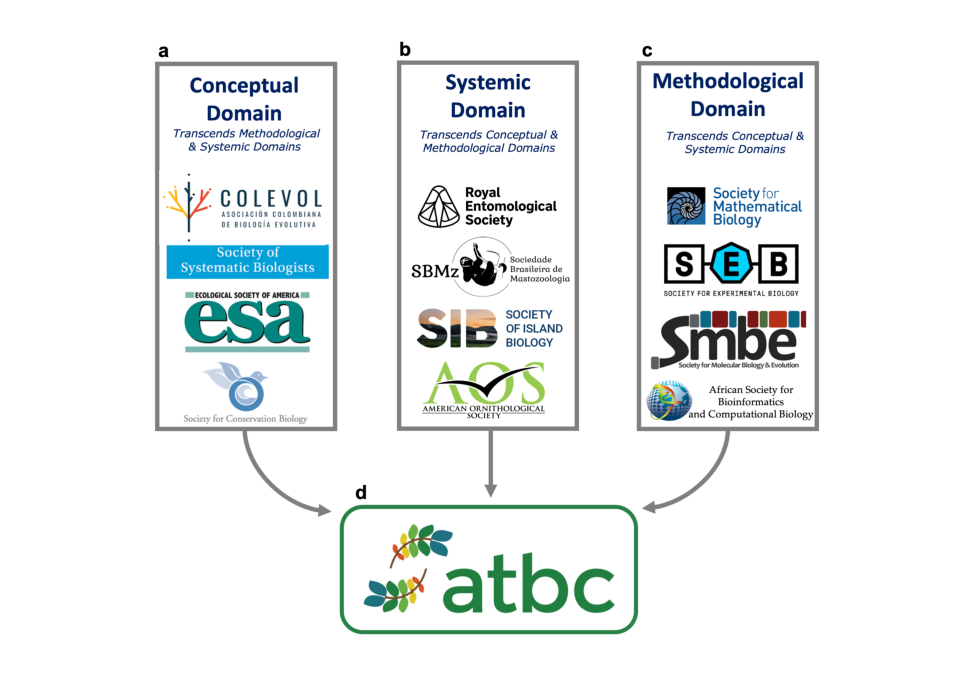
\includegraphics[width=1\linewidth,height=0.9\textheight,]{Bruna_plenary_MS_files/figure-latex/fig-org-1} 

}

\caption{Alternative ways in which researchers self-organize in scholarly societies: (a) Conceptual Domain, (b) Systemic Domain, or (c) Methodological Domain. The Association for Tropical Biology \& Conservation (i.e., ATBC) is unique in that transcends the three domains: its members use a broad diversity of species, ecosystems, and methods to address questions grounded in -- or even transcending -- multiple distinct conceptual domains.}\label{fig:fig-org}
\end{figure}

\newpage

\begin{figure}[H]

{\centering 
\includegraphics[width=1\linewidth,height=0.8\textheight,]{Bruna_plenary_MS_files/figure-latex/fig-temp-1} 

}

\caption{The logo for a proposed new scholarly society for researchers specializing on temperate ecosystems and species.}\label{fig:fig-temp}
\end{figure}

\newpage

\begin{figure}[H]

{\centering 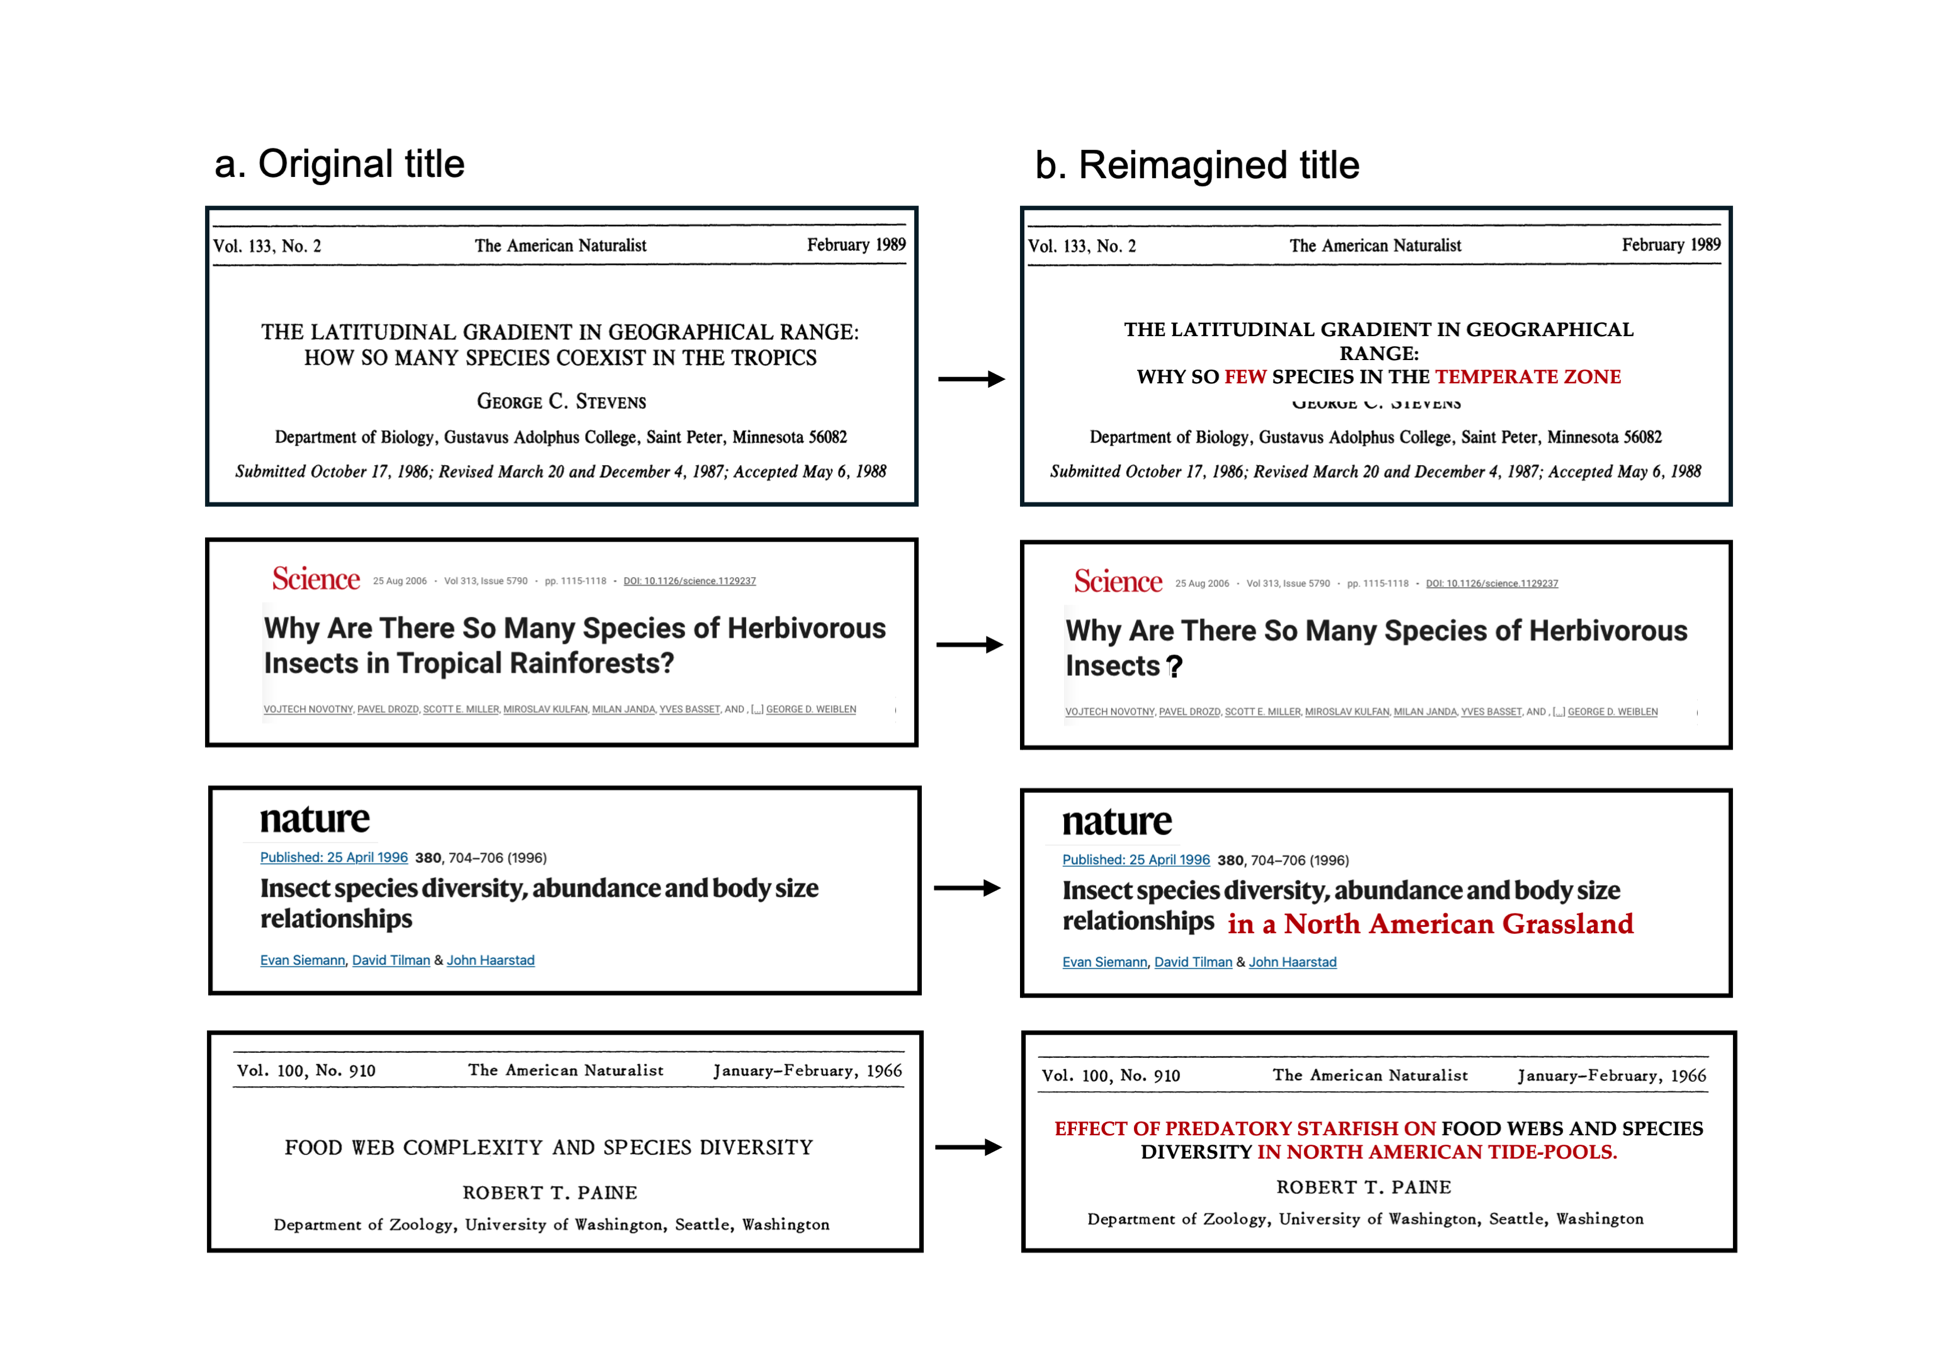
\includegraphics[width=1\linewidth,height=1\textheight,]{Bruna_plenary_MS_files/figure-latex/fig-pubs-1} 

}

\caption{The (a) original and (b) reimagined titles of four high-profile research articles. Comparing these emphasizes how the original titles reflect and reinforce the idea that 'reference' or 'default ecosystems are found in the Temperate Zone.}\label{fig:fig-pubs}
\end{figure}
\newpage

\hypertarget{acknowldgements}{%
\subsection{ACKNOWLDGEMENTS}\label{acknowldgements}}

I am grateful to the organizers of the 2022 Meeting of the ATBC for encouraging the Presidential Plenary on which this essay is based, to J. Powers for her outstanding editorial work, and to P. Delamônica for her unending support and insights. I am also grateful to M. Raby and N. Stepan, whose outstanding books shaped many of the ideas expressed here. This essay is dedicated to the memory of Emilio Bruna Jr.

\hypertarget{data-availability-statement}{%
\subsection{DATA AVAILABILITY STATEMENT}\label{data-availability-statement}}

The complete data set used in this article is available in Dryad at \textless{}\emph{DOI added upon acceptance}\textgreater. The version of the code used to review, correct, and prepare the data archive (v1.0.0) is available at Zenodo at \textless{}\emph{DOI added upon acceptance}\textgreater. The code used to prepare this publication, including statistical summaries reported in the text, tables, and figures, is available at Zenodo at \textless{}\emph{DOI added upon acceptance}\textgreater. Questions regarding the data or code, or suggestions for improvement should be posted as Issues on the project's Github Repository (\url{https://github.com/BrunaLab/atbc2022_plenary_talk}) or referred to E. M. Bruna. Summaries of any post-publication updates will be posted to the NEWS.md file of this Github Repository.

\hypertarget{disclosure-statement}{%
\subsection{DISCLOSURE STATEMENT}\label{disclosure-statement}}

The author confirms that there have been no involvements that might raise the question of bias in the work reported or in the conclusions, implications, or opinions stated.

\hypertarget{author-contribution-statement}{%
\subsection{AUTHOR CONTRIBUTION STATEMENT}\label{author-contribution-statement}}

E.M.B conceived the study and is responsible for the methodology, data collection, data curation, formal analysis, validation, visualization, software, and writing.

\newpage

\hypertarget{references}{%
\section{REFERENCES}\label{references}}

\hypertarget{refs}{}
\begin{CSLReferences}{1}{0}
\leavevmode\vadjust pre{\hypertarget{ref-albertTwentyMostCharismatic2018}{}}%
\textsc{Albert, C.}, \textsc{G. M. Luque}, and \textsc{F. Courchamp}. 2018. \href{https://doi.org/10.1371/journal.pone.0199149}{The twenty most charismatic species}. PLOS ONE 13: e0199149.

\leavevmode\vadjust pre{\hypertarget{ref-amanoLanguagesAreStill2016}{}}%
\textsc{Amano, T.}, \textsc{J. P. González-Varo}, and \textsc{W. J. Sutherland}. 2016. \href{https://doi.org/10.1371/journal.pbio.2000933}{Languages are still a major barrier to global science}. PLoS Biology 14: e2000933.

\leavevmode\vadjust pre{\hypertarget{ref-andersonTrendsEcologyConservation2021}{}}%
\textsc{Anderson, S. C.}, \textsc{P. R. Elsen}, \textsc{B. B. Hughes}, \textsc{R. K. Tonietto}, \textsc{M. C. Bletz}, \textsc{D. A. Gill}, \textsc{M. A. Holgerson}, \textsc{S. E. Kuebbing}, \textsc{C. McDonough MacKenzie}, \textsc{M. H. Meek}, and \textsc{D. Veríssimo}. 2021. \href{https://doi.org/10.1002/fee.2320}{Trends in ecology and conservation over eight decades}. Frontiers in Ecology and the Environment 19: 274--282.

\leavevmode\vadjust pre{\hypertarget{ref-annanChallengeWorldScientists2003}{}}%
\textsc{Annan, K.} 2003. \href{https://doi.org/10.1126/science.299.5612.1485}{A challenge to the world's scientists}. Science 299: 1485--1485.

\leavevmode\vadjust pre{\hypertarget{ref-arnold1996problem}{}}%
\textsc{Arnold, D.} 1996. The problem of nature: {Environment}, culture and {European} expansion. Blackwell.

\leavevmode\vadjust pre{\hypertarget{ref-asaseReplacingParachuteScience2022}{}}%
\textsc{Asase, A.}, \textsc{T. I. Mzumara-Gawa}, \textsc{J. O. Owino}, \textsc{A. T. Peterson}, and \textsc{E. Saupe}. 2022. \href{https://doi.org/10.1111/csp2.517}{Replacing {``parachute science''} with {``global science''} in ecology and conservation biology}. Conservation Science and Practice 4: e517.

\leavevmode\vadjust pre{\hypertarget{ref-bairleinCrosshemisphereMigration252012}{}}%
\textsc{Bairlein, F.}, \textsc{D. R. Norris}, \textsc{R. Nagel}, \textsc{M. Bulte}, \textsc{C. C. Voigt}, \textsc{J. W. Fox}, \textsc{D. J. T. Hussell}, and \textsc{H. Schmaljohann}. 2012. \href{https://doi.org/10.1098/rsbl.2011.1223}{Cross-hemisphere migration of a 25 g songbird}. Biology Letters 8: 505--507.

\leavevmode\vadjust pre{\hypertarget{ref-bassetConservationBiologicalMonitoring2004}{}}%
\textsc{Basset, Y.}, \textsc{V. Novotny}, \textsc{S. E. Miller}, \textsc{G. D. Weiblen}, \textsc{O. Missa}, and \textsc{A. J. A. Stewart}. 2004. Conservation and biological monitoring of tropical forests: The role of parataxonomists. Journal of Applied Ecology 41: 163--174.

\leavevmode\vadjust pre{\hypertarget{ref-bawaParadiseMeetingChallenges2004}{}}%
\textsc{Bawa, K. S.}, \textsc{W. J. Kress}, \textsc{N. M. Nadkarni}, and \textsc{S. Lele}. 2004. \href{https://doi.org/10.1111/j.1744-7429.2004.tb00341.x}{Beyond paradise: Meeting the challenges in tropical biology in the 21st century}. Biotropica 36: 437--446.

\leavevmode\vadjust pre{\hypertarget{ref-benoitStopwordsMultilingualStopword2021}{}}%
\textsc{Benoit, K.}, \textsc{D. Muhr}, and \textsc{K. Watanabe}. 2021. Stopwords: {Multilingual} stopword lists.

\leavevmode\vadjust pre{\hypertarget{ref-brunaHeliconiaAcuminataReproductive2004e}{}}%
\textsc{Bruna, E. M.}, \textsc{W. J. Kress}, \textsc{F. Marques}, and \textsc{O. F. da Silva}. 2004.\href{https://doi.org/10.1590/S0044-59672004000300012}{{ \emph{Heliconia Acuminata} } reproductive success is independent of local floral density}. Acta Amazonica 34: 467--471.

\leavevmode\vadjust pre{\hypertarget{ref-buechnerContributionWorldProgram1967}{}}%
\textsc{Buechner, H. K.}, and \textsc{F. R. Fosberg}. 1967. \href{https://doi.org/10.2307/1294010}{A contribution toward a world program in tropical biology}. BioScience 17: 532--538.

\leavevmode\vadjust pre{\hypertarget{ref-carmelTrendsEcologicalResearch2013}{}}%
\textsc{Carmel, Y.}, \textsc{R. Kent}, \textsc{A. Bar-Massada}, \textsc{L. Blank}, \textsc{J. Liberzon}, \textsc{O. Nezer}, \textsc{G. Sapir}, and \textsc{R. Federman}. 2013. \href{https://doi.org/10.1371/journal.pone.0059813}{Trends in ecological research during the last three decades: A systematic review}. PLoS ONE 8: e59813.

\leavevmode\vadjust pre{\hypertarget{ref-castrotorresNorthSouthNaming2022}{}}%
\textsc{Castro Torres, A. F.}, and \textsc{D. Alburez-Gutierrez}. 2022. \href{https://doi.org/10.1073/pnas.2119373119}{North and {South}: {Naming} practices and the hidden dimension of global disparities in knowledge production}. Proceedings of the National Academy of Sciences 119: e2119373119.

\leavevmode\vadjust pre{\hypertarget{ref-cavalcantiPoliticalViolenceMobilisation2023}{}}%
\textsc{Cavalcanti, R. P.}, \textsc{G. F. Benzaquen}, \textsc{S. da S. R. Gomes}, and \textsc{V. P. Almeida}. 2023. \href{https://doi.org/10.1332/SONH8866}{Political violence and mobilisation in {Brazil}'s {Amazonian} region during {Bolsonaro}'s government (2019--2022)}. Justice, Power and Resistance 6: 152--170.

\leavevmode\vadjust pre{\hypertarget{ref-chapmanNeedDevelopmentTropical1945}{}}%
\textsc{Chapman, V. J.}, \textsc{C. O. Flemmich}, \textsc{A. L. Griffith}, \textsc{J. L. Harley}, \textsc{R. Hobbins}, \textsc{C. H. Holmes}, \textsc{C. De Rosayro}, and \textsc{J. Wyatt-Smith}. 1945. \href{https://doi.org/10.1038/156627a0}{Need for development of tropical ecological studies}. Nature 156: 627--628.

\leavevmode\vadjust pre{\hypertarget{ref-chazdonFoundationsTropicalForest2001}{}}%
\textsc{Chazdon, R. L.}, and \textsc{T. C. Whitmore} eds. 2001. Foundations of {Tropical Forest Biology}: {Classic Papers} with {Commentaries}. University of Chicago Press, Chicago, IL.

\leavevmode\vadjust pre{\hypertarget{ref-clancySurveyAcademicField2014}{}}%
\textsc{Clancy, K. B. H.}, \textsc{R. G. Nelson}, \textsc{J. N. Rutherford}, and \textsc{K. Hinde}. 2014. \href{https://doi.org/10.1371/journal.pone.0102172}{Survey of academic field experiences ({SAFE}): Trainees report harassment and assault}. PLoS ONE 9: e102172.

\leavevmode\vadjust pre{\hypertarget{ref-cornerNeedDevelopmentTropical1946}{}}%
\textsc{Corner, E. J. H.} 1946. \href{https://doi.org/10.1038/157377b0}{Need for the development of tropical ecological stations}. Nature 157: 377--377.

\leavevmode\vadjust pre{\hypertarget{ref-driverConstructingTropicsIntroduction2000}{}}%
\textsc{Driver, F.}, and \textsc{B. S. A. Yeoh}. 2000. \href{https://doi.org/10.1111/1467-9493.00059}{Constructing the tropics: introduction}. Singapore Journal of Tropical Geography 21: 1--5.

\leavevmode\vadjust pre{\hypertarget{ref-duchelleGraduateStudentsKnowledge2009}{}}%
\textsc{Duchelle, A. E.}, \textsc{K. Biedenweg}, \textsc{C. Lucas}, \textsc{A. Virapongse}, \textsc{J. Radachowsky}, \textsc{D. J. Wojcik}, \textsc{M. Londres}, \textsc{W.-L. Bartels}, \textsc{D. Alvira}, and \textsc{K. A. Kainer}. 2009. \href{https://doi.org/10.1111/j.1744-7429.2009.00563.x}{Graduate students and knowledge exchange with local stakeholders: Possibilities and preparation}. Biotropica 41: 578--585.

\leavevmode\vadjust pre{\hypertarget{ref-ellwangerDiversityLossClimate2020}{}}%
\textsc{Ellwanger, J. H.}, \textsc{B. Kulmann-Leal}, \textsc{V. L. Kaminski}, \textsc{J. M. Valverde-Villegas}, \textsc{A. B. G. D. Veiga}, \textsc{F. R. Spilki}, \textsc{P. M. Fearnside}, \textsc{L. Caesar}, \textsc{L. L. Giatti}, \textsc{G. L. Wallau}, \textsc{S. E. M. Almeida}, \textsc{M. R. Borba}, \textsc{V. P. D. Hora}, and \textsc{J. A. B. Chies}. 2020. \href{https://doi.org/10.1590/0001-3765202020191375}{Beyond diversity loss and climate change: {Impacts} of {Amazon} deforestation on infectious diseases and public health}. Anais da Academia Brasileira de Ci{ê}ncias 92: e20191375.

\leavevmode\vadjust pre{\hypertarget{ref-eppleyTropicalFieldStations2024}{}}%
\textsc{Eppley, T. M.} et al. 2024. \href{https://doi.org/10.1111/conl.13007}{Tropical field stations yield high conservation return on investment}. Conservation Letters e13007.

\leavevmode\vadjust pre{\hypertarget{ref-fournierRefsplitrAuthorName2020}{}}%
\textsc{Fournier, A. M. V.}, \textsc{M. E. Boone}, \textsc{F. R. Stevens}, and \textsc{E. M. Bruna}. 2020. \href{https://doi.org/10.21105/joss.02028}{Refsplitr: {Author} name disambiguation, author georeferencing, and mapping of coauthorship networks with {Web} of {Science} data}. Journal of Open Source Software 5: 2028.

\leavevmode\vadjust pre{\hypertarget{ref-gastonGlobalPatternsBiodiversity2000}{}}%
\textsc{Gaston, K. J.} 2000. \href{https://doi.org/10.1038/35012228}{Global patterns in biodiversity}. Nature 405: 220--227.

\leavevmode\vadjust pre{\hypertarget{ref-gomez-pompaRoleBiodiversityScientists2004}{}}%
\textsc{Gómez-Pompa, A.} 2004. \href{https://doi.org/10.1641/0006-3568(2004)054\%5B0217:TROBSI\%5D2.0.CO;2}{The role of biodiversity scientists in a troubled world}. BioScience 54: 217--225.

\leavevmode\vadjust pre{\hypertarget{ref-alma9913280634202441}{}}%
\textsc{Gourou, P.} 1947. {Les pays tropicaux, principes d'une g{é}ographie humaine et {é}conomique.} {[}1. {é}d.{]}. Presses Universitaires de France, Paris.

\leavevmode\vadjust pre{\hypertarget{ref-hoornwegPopulationPredictionsWorld2017}{}}%
\textsc{Hoornweg, D.}, and \textsc{K. Pope}. 2017. \href{https://doi.org/10.1177/0956247816663557}{Population predictions for the world's largest cities in the 21st century}. Environment and Urbanization 29: 195--216.

\leavevmode\vadjust pre{\hypertarget{ref-janzenWhitherTropicalEcology1972}{}}%
\textsc{Janzen, D.} 1972. Whither {Tropical Ecology}. \emph{In} J. A. Behnke (Ed.) Challenging {Biological Problems}: {Directions Toward Their Solution}. pp. 281--296, Oxford University Press, New York.

\leavevmode\vadjust pre{\hypertarget{ref-janzenFutureTropicalEcology1986}{}}%
\textsc{Janzen, D. H.} 1986. The future of tropical ecology. Annual Review of Ecology and Systematics 17: 305--324.

\leavevmode\vadjust pre{\hypertarget{ref-kainerPartneringGreaterSuccess2009}{}}%
\textsc{Kainer, K. A.}, \textsc{M. L. DiGiano}, \textsc{A. E. Duchelle}, \textsc{L. H. O. Wadt}, \textsc{E. M. Bruna}, and \textsc{J. L. Dain}. 2009. \href{https://doi.org/10.1111/j.1744-7429.2009.00560.x}{Partnering for greater success: Local stakeholders and research in tropical biology and conservation}. Biotropica 41: 555--562.

\leavevmode\vadjust pre{\hypertarget{ref-kainerGraduateEducationFramework2006}{}}%
\textsc{Kainer, K. A.}, \textsc{M. Schmink}, \textsc{H. Covert}, \textsc{J. R. Stepp}, \textsc{E. M. Bruna}, \textsc{J. L. Dain}, \textsc{S. Espinosa}, and \textsc{S. Humphries}. 2006. \href{https://doi.org/10.1111/j.1523-1739.2006.00356.x}{A graduate education framework for tropical conservation and development}. Conservation Biology 20: 3--13.

\leavevmode\vadjust pre{\hypertarget{ref-kuteskoAdidasShowsChanging2014}{}}%
\textsc{Kutesko, E.} 2014. Adidas shows the changing face of {Brazil} with tropical collection. The Conversation (available at http://theconversation.com/adidas-shows-the-changing-face-of-brazil-with-tropical-collection-26546).

\leavevmode\vadjust pre{\hypertarget{ref-mccallenTrendsEcologyShifts2019}{}}%
\textsc{McCallen, E.}, \textsc{J. Knott}, \textsc{G. Nunez-Mir}, \textsc{B. Taylor}, \textsc{I. Jo}, and \textsc{S. Fei}. 2019. \href{https://doi.org/10.1002/fee.1993}{Trends in ecology: Shifts in ecological research themes over the past four decades}. Frontiers in Ecology and the Environment 17: 109--116.

\leavevmode\vadjust pre{\hypertarget{ref-meloFootballBiodiversityConservation2014}{}}%
\textsc{Melo, F. P.}, \textsc{J. A. Siqueira}, \textsc{B. A. Santos}, \textsc{O. Álvares-da-Silva}, \textsc{G. Ceballos}, and \textsc{E. Bernard}. 2014. \href{https://doi.org/10.1111/btp.12114}{{Football and biodiversity conservation: FIFA and Brazil can still hit a green goal}}. Biotropica 46: 257--259.

\leavevmode\vadjust pre{\hypertarget{ref-miller2011visions}{}}%
\textsc{Miller, D. P.}, and \textsc{P. H. Reill} eds. 2011. Visions of empire: Voyages, botany, and representations of nature. Cambridge University Press.

\leavevmode\vadjust pre{\hypertarget{ref-molesNotionThatSpecies2016}{}}%
\textsc{Moles, A. T.}, and \textsc{J. Ollerton}. 2016. \href{https://doi.org/10.1111/btp.12281}{Is the notion that species interactions are stronger and more specialized in the tropics a zombie idea?} Biotropica 48: 141--145.

\leavevmode\vadjust pre{\hypertarget{ref-moreiraTamarProjectConservation2017}{}}%
\textsc{Moreira, J. C.}, and \textsc{R. A. Robles}. 2017. \href{https://doi.org/10.1007/978-3-319-55574-4_10}{Tamar {Project}: Conservation and education in ecotourism activities related to turtles in {Fernando} de {Noronha Archipelago}, {Brazil}}. \emph{In} I. Borges de Lima and R. J. Green (Eds.) Wildlife {Tourism}, {Environmental Learning} and {Ethical Encounters}: {Ecological} and {Conservation Aspects}. Geoheritage, {Geoparks} and {Geotourism}. pp. 169--181, Springer International Publishing, Cham.

\leavevmode\vadjust pre{\hypertarget{ref-nordsethFieldworkWellnessFramework2023}{}}%
\textsc{Nordseth, A. E.}, \textsc{J. R. Gerson}, \textsc{L. K. Aguilar}, \textsc{A. E. Dunham}, \textsc{A. Gentles}, \textsc{Z. Neale}, and \textsc{E. Rebol}. 2023. \href{https://doi.org/10.1002/fee.2649}{The {Fieldwork Wellness Framework}: A new approach to field research in ecology}. Frontiers in Ecology and the Environment 21: 297--303.

\leavevmode\vadjust pre{\hypertarget{ref-ocampo-arizaGlobalSouthLeadership2023}{}}%
\textsc{Ocampo-Ariza, C.} et al. 2023. \href{https://doi.org/10.1016/j.pecon.2023.01.002}{Global {South} leadership towards inclusive tropical ecology and conservation}. Perspectives in Ecology and Conservation 21: 17--24.

\leavevmode\vadjust pre{\hypertarget{ref-palinkasGlobalClimateChange2020}{}}%
\textsc{Palinkas, L. A.}, and \textsc{M. Wong}. 2020. \href{https://doi.org/10.1016/j.copsyc.2019.06.023}{Global climate change and mental health}. Current Opinion in Psychology 32: 12--16.

\leavevmode\vadjust pre{\hypertarget{ref-parkObservationsConcerningFuture1945}{}}%
\textsc{Park, O.} 1945. \href{https://doi.org/10.2307/1931910}{Observations concerning the future of ecology}. Ecology 26: 1--9.

\leavevmode\vadjust pre{\hypertarget{ref-inbook}{}}%
\textsc{Putz, F. E.}, and \textsc{N. M. Holbrook}. 1988. Tropical rain-forest images. \emph{In} J. S. Denslow and C. Padoch (Eds.) People of the {Tropical Rain Forest}. pp. 37--52, University of California Press, Berkeley.

\leavevmode\vadjust pre{\hypertarget{ref-rcoreteamLanguageEnvironmentStatistical2023}{}}%
\textsc{R Core Team}. 2023. R: {A} language and environment for statistical computing. R Foundation for Statistical Computing, Vienna, Austria.

\leavevmode\vadjust pre{\hypertarget{ref-raby2017american}{}}%
\textsc{Raby, M.} 2017a. American tropics: The {Caribbean} roots of biodiversity science. UNC Press Books.

\leavevmode\vadjust pre{\hypertarget{ref-rabyColonialOriginsTropical2017}{}}%
\textsc{Raby, M.} 2017b. The colonial origins of tropical field stations: To confront persistent geographic and demographic biases in environmental science, researchers must understand the history of their field sites. American Scientist 105: 216--224.

\leavevmode\vadjust pre{\hypertarget{ref-ramirez-castanedaSetPrinciplesPractical2022}{}}%
\textsc{Ramírez-Castañeda, V.} et al. 2022. \href{https://doi.org/10.1073/pnas.2122667119}{A set of principles and practical suggestions for equitable fieldwork in biology}. Proceedings of the National Academy of Sciences 119: e2122667119.

\leavevmode\vadjust pre{\hypertarget{ref-richardsNeedDevelopmentTropical1946}{}}%
\textsc{Richards, P. W.} 1946. \href{https://doi.org/10.1038/157377a0}{Need for the development of tropical ecological stations}. Nature 157: 377--377.

\leavevmode\vadjust pre{\hypertarget{ref-richardsWhatTropicsCan1963}{}}%
\textsc{Richards, P. W.} 1963. \href{https://doi.org/10.2307/2257682}{What the tropics can contribute to ecology}. Journal of Ecology 51: 231--241.

\leavevmode\vadjust pre{\hypertarget{ref-richardsProgrammeTropicalBiology1964}{}}%
\textsc{Richards, P. W.} 1964. Towards a programme for tropical biology. Bulletin of the Association for Tropical Biology 8--15.

\leavevmode\vadjust pre{\hypertarget{ref-ripleyPerspectivesTropicalBiology1967}{}}%
\textsc{Ripley, S. D.} 1967. \href{https://doi.org/10.2307/1294011}{Perspectives in tropical biology}. BioScience 17: 538--540.

\leavevmode\vadjust pre{\hypertarget{ref-robinson1978tropical}{}}%
\textsc{Robinson, M. H.} 1978. Is tropical biology real. Tropical Ecology 19: 30--52.

\leavevmode\vadjust pre{\hypertarget{ref-rudzkiGuideDevelopingField2022}{}}%
\textsc{Rudzki, E. N.}, \textsc{S. E. Kuebbing}, \textsc{D. R. Clark}, \textsc{B. Gharaibeh}, \textsc{M. J. Janecka}, \textsc{R. Kramp}, \textsc{K. D. Kohl}, \textsc{T. Mastalski}, \textsc{M. E. B. Ohmer}, \textsc{M. M. Turcotte}, and \textsc{C. L. Richards-Zawacki}. 2022. \href{https://doi.org/10.1111/2041-210X.13970}{A guide for developing a field research safety manual that explicitly considers risks for marginalized identities in the sciences}. Methods in Ecology and Evolution 13: 2318--2330.

\leavevmode\vadjust pre{\hypertarget{ref-russellIntegratingTropicalResearch2022}{}}%
\textsc{Russell, A. E.}, \textsc{T. M. Aide}, \textsc{E. Braker}, \textsc{C. N. Ganong}, \textsc{R. D. Hardin}, \textsc{K. D. Holl}, \textsc{S. C. Hotchkiss}, \textsc{J. A. Klemens}, \textsc{E. K. Kuprewicz}, \textsc{D. McClearn}, \textsc{G. Middendorf}, \textsc{R. Ostertag}, \textsc{J. S. Powers}, \textsc{S. E. Russo}, \textsc{J. L. Stynoski}, \textsc{U. Valdez}, and \textsc{C. G. Willis}. 2022. \href{https://doi.org/10.1371/journal.pbio.3001674}{Integrating tropical research into biology education is urgently needed}. PLoS Biology 20: e3001674.

\leavevmode\vadjust pre{\hypertarget{ref-sartore-baldwinExaminingSportFans2019}{}}%
\textsc{Sartore-Baldwin, M.}, and \textsc{B. McCullough}. 2019. \href{https://doi.org/10.1163/15685306-12341605}{Examining sport fans and the endangered species who represent their affiliated team mascots}. Society \& Animals 29: 268--286.

\leavevmode\vadjust pre{\hypertarget{ref-silgeTidytextTextMining2016}{}}%
\textsc{Silge, J.}, and \textsc{D. Robinson}. 2016. \href{https://doi.org/10.21105/joss.00037}{Tidytext: {Text} mining and analysis using tidy data principles in {R}}. Journal of Open Source Software 1(3).

\leavevmode\vadjust pre{\hypertarget{ref-smithAssessingEffectArticle2021}{}}%
\textsc{Smith, A. C.}, \textsc{L. Merz}, \textsc{J. B. Borden}, \textsc{C. K. Gulick}, \textsc{A. R. Kshirsagar}, and \textsc{E. M. Bruna}. 2021. \href{https://doi.org/10.1162/qss_a_00157}{Assessing the effect of article processing charges on the geographic diversity of authors using {Elsevier}'s {``{Mirror Journal}''} system}. Quantitative Science Studies 2: 1123--1143.

\leavevmode\vadjust pre{\hypertarget{ref-smithEuropeanVisionSouth1950}{}}%
\textsc{Smith, B.} 1950. \href{https://doi.org/10.2307/750143}{European vision and the {South Pacific}}. Journal of the Warburg and Courtauld Institutes 13: 65--100.

\leavevmode\vadjust pre{\hypertarget{ref-smithScientificImpactNations2014}{}}%
\textsc{Smith, M. J.}, \textsc{C. Weinberger}, \textsc{E. M. Bruna}, and \textsc{S. Allesina}. 2014. \href{https://doi.org/10.1371/journal.pone.0109195}{The scientific impact of nations: Journal placement and citation performance}. PLoS ONE 9.

\leavevmode\vadjust pre{\hypertarget{ref-smithPeerReviewPerpetuates2023}{}}%
\textsc{Smith, O. M.}, \textsc{K. L. Davis}, \textsc{R. B. Pizza}, \textsc{R. Waterman}, \textsc{K. C. Dobson}, \textsc{B. Foster}, \textsc{J. C. Jarvey}, \textsc{L. N. Jones}, \textsc{W. Leuenberger}, \textsc{N. Nourn}, \textsc{E. E. Conway}, \textsc{C. M. Fiser}, \textsc{Z. A. Hansen}, \textsc{A. Hristova}, \textsc{C. Mack}, \textsc{A. N. Saunders}, \textsc{O. J. Utley}, \textsc{M. L. Young}, and \textsc{C. L. Davis}. 2023. \href{https://doi.org/10.1038/s41559-023-01999-w}{Peer review perpetuates barriers for historically excluded groups}. Nature Ecology \& Evolution 7: 512--523.

\leavevmode\vadjust pre{\hypertarget{ref-sohmerNSFSupportBasic1980}{}}%
\textsc{Sohmer, S. H.} 1980. \href{https://doi.org/10.2307/1308006}{{NSF} support of basic research in tropical biology}. BioScience 30: 412--415.

\leavevmode\vadjust pre{\hypertarget{ref-stegmannBrazilianPublicFunding2024}{}}%
\textsc{Stegmann, L. F.}, \textsc{F. M. França}, \textsc{R. L. Carvalho}, \textsc{J. Barlow}, \textsc{E. Berenguer}, \textsc{L. Castello}, \textsc{L. Juen}, \textsc{F. B. Baccaro}, \textsc{I. C. G. Vieira}, \textsc{C. A. Nunes}, \textsc{R. Oliveira}, \textsc{E. M. Venticinque}, \textsc{J. Schietti}, and \textsc{J. Ferreira}. 2024. \href{https://doi.org/10.1016/j.pecon.2024.01.003}{Brazilian public funding for biodiversity research in the {Amazon}}. Perspectives in Ecology and Conservation 22: 1--7.

\leavevmode\vadjust pre{\hypertarget{ref-stepan2001picturing}{}}%
\textsc{Stepan, N.} 2001. Picturing tropical nature. Cornell University Press, Ithaca.

\leavevmode\vadjust pre{\hypertarget{ref-stocksGeographicalInstitutionalDistribution2008}{}}%
\textsc{Stocks, G.}, \textsc{L. Seales}, \textsc{F. Paniagua}, \textsc{E. Maehr}, and \textsc{E. M. Bruna}. 2008. \href{https://doi.org/10.1111/j.1744-7429.2007.00393.x}{The geographical and institutional distribution of ecological research in the tropics}. Biotropica 40: 397--404.

\leavevmode\vadjust pre{\hypertarget{ref-unescoSixtyYearsScience2006}{}}%
\textsc{Unesco} ed. 2006. Sixty years of science at {UNESCO} 1945-2005. UNESCO Pub, Paris.

\leavevmode\vadjust pre{\hypertarget{ref-vandresserFutureAmazon1948}{}}%
\textsc{van Dresser, P.} 1948. The {Future} of the {Amazon}. Scientific American 178: 11--15.

\leavevmode\vadjust pre{\hypertarget{ref-webbBiologyTropics1960}{}}%
\textsc{Webb, J. E.} 1960. \href{https://doi.org/10.1038/188617a0}{Biology in the {Tropics}}. Nature 188: 617--619.

\leavevmode\vadjust pre{\hypertarget{ref-yongReelConservationCan2011}{}}%
\textsc{Yong, D. L.}, \textsc{S. D. Fam}, and \textsc{S. Lum}. 2011. \href{https://doi.org/10.1177/194008291100400302}{Reel conservation: {Can} big screen animations save tropical biodiversity?} Tropical Conservation Science 4: 244--253.

\leavevmode\vadjust pre{\hypertarget{ref-zukTemperateAssumptionsHow2016}{}}%
\textsc{Zuk, M.} 2016. \href{https://doi.org/10.1086/687546}{Temperate assumptions: How where we work influences how we think}. The American Naturalist 188: S1--S7.

\end{CSLReferences}

\newpage

\renewcommand{\appendixname}{Supporting Information}
\renewcommand{\thefigure}{S\arabic{figure}} \setcounter{figure}{0}
\renewcommand{\thetable}{S\arabic{table}} \setcounter{table}{0}
\renewcommand{\theequation}{S\arabic{table}} \setcounter{equation}{0}
\setcounter{page}{1}

\nolinenumbers

\hypertarget{supporting-information}{%
\section{SUPPORTING INFORMATION}\label{supporting-information}}

\bigskip
\bigskip

\hypertarget{is-there-really-such-a-thing-as-tropical-biology}{%
\subsection{\texorpdfstring{Is there really such a thing as \emph{Tropical} Biology?}{Is there really such a thing as Tropical Biology?}}\label{is-there-really-such-a-thing-as-tropical-biology}}

\bigskip
\bigskip
\bigskip
\bigskip

\noindent Emilio M. Bruna \textsuperscript{1,2} \(^\ast\)

\bigskip
\bigskip

\noindent \textsuperscript{1} Department of Wildlife Ecology and Conservation, University of Florida, PO Box 110430, Gainesville, FL 32611-0430, USA

\noindent \textsuperscript{2} Center for Latin American Studies, University of Florida, PO Box 115530, Gainesville, FL 32611-5530, USA

\bigskip

\noindent \(^\ast\) Corresponding author; email: \href{mailto:embruna@ufl.edu}{\nolinkurl{embruna@ufl.edu}}.

\newpage
\resetlinenumber
\linenumbers

\hypertarget{collection-processing-and-visualization-of-bibliometric-data}{%
\subsection{1. Collection, processing, and visualization of bibliometric data}\label{collection-processing-and-visualization-of-bibliometric-data}}

\noindent To identify the conceptual domains studied by researchers working in `Tropical' and ``non-Tropical' locations, I used information extracted from the bibliographic records of articles published These studies were published from 1990-2022 in N = 10 journals (\emph{Journal of Evolutionary Biology, Ecology, Journal of Applied Ecology, Evolution, Biotropica, Journal of Ecology, Tropical Conservation Science, American Naturalist, Tropical Ecology, Journal of Tropical Ecology}). Specifically, I compared (1) article keywords, (2) individual words in article titles (e.g., \emph{seed}, \emph{species}), and (3) title bigrams (i.e., pairs of sequential words in titles, e.g., \emph{seed predation}, \emph{species diversity}). Below I describe how the article records were identified, downloaded, processed, and assigned to the `Tropical' and''non-Tropical' categories using code written in the \texttt{R} programming language (R Core Team 2023).\\
On 8 February 2023, I downloaded all bibliographic data available in SCOPUS and the Web of Science `Core Collection' for all articles published in the focal journals; both SCOPUS and the Web of Science were queried because they differ in the years indexed for each journal. I then used the \texttt{refsplitr} package (Fournier \emph{et al.} 2020) to process the records and remove any duplicates. After removing all stopwords (Benoit \emph{et al.} 2021) from article titles and keywords, I spell-checked, stemmed, and lemmatized all of the keywords and title words. I also extracted bigrams from titles with the \texttt{tidytext} library (Silge \& Robinson 2016). Finally, I identified each article as either `Tropical' or `non-Tropical'; all articles published in (\emph{Journal of Evolutionary Biology, Ecology, Journal of Applied Ecology, Evolution, Biotropica, Journal of Ecology, Tropical Conservation Science, American Naturalist, Tropical Ecology, Journal of Tropical Ecology}) were assigned to the `Tropical' category, while articles published in the other journals were assigned to one of these categories based on a search of the titles, keywords, or abstracts for a list of domain-specific terms (e.g., tropical: \emph{amazon}, \emph{andes}, \emph{congo}, \emph{bci}, \emph{chamela}; non-tropical: \emph{finland}, \emph{boreal}, \emph{eastern decid}, \emph{arctic}, \emph{polar}). These procedures resulted in N = 37,807 total articles published, of which N = 11,210 reported research conducted in the tropics and N = 26,597 were based on work conducted in other locations. Collectively, these articles used N = 62,883, N = 25,207 unique title words, and N = 126,796 title bigrams.\\
The number of articles varies widely between journals, as does the number of keywords per article. Comparing counts of keyword frequency in tropical and non-tropical articles could therefore bias results towards the content published a small number of journals. To correct for this, I calculated the percentage of articles in each geographic category that uising each keyword, title word, or bigram. I then selected the N = 50 most frequently used terms in each geographic category, and identified (a) any terms that `tropical' and `non-tropical' articles had in common, and (b) any terms that were unique to each article category.

\hypertarget{data-and-code}{%
\subsection{2. Data and Code}\label{data-and-code}}

\noindent The version of the code used to review, correct, and prepare the data set (version 1.0.0) is available at Zenodo at \textless{}\emph{DOI added upon acceptance}\textgreater, and the data set used in this publication is available in Dryad at \textless{}\emph{DOI added upon acceptance}\textgreater. The code used to prepare this publication, including statistical summaries reported in the text, tables, and figures, is also available at Zenodo at \textless{}\emph{DOI added upon acceptance}\textgreater. Questions regarding the data or code, or suggestions for improvement should be posted as Issues on the project's Github Repository (\url{https://github.com/BrunaLab/atbc2022_plenary_talk}) or referred to E. M. Bruna. Summaries of any post-publication updates will be posted to the NEWS.md file of this Github Repository.

\hypertarget{references-1}{%
\subsection{REFERENCES}\label{references-1}}

\textsc{Benoit, K.}, \textsc{D. Muhr}, and \textsc{K. Watanabe}. 2021. Stopwords: Multilingual stopword lists. \url{https://CRAN.R-project.org/package=stopwords}

\textsc{Fournier, A. M. V.}, \textsc{M. E. Boone}, \textsc{F. R. Stevens}, and \textsc{E. M. Bruna}. 2020. \href{https://doi.org/10.21105/joss.02028}{Refsplitr: Author name disambiguation, author georeferencing, and mapping of coauthorship networks with Web of Science data}. Journal of Open Source Software 5: 2028.

\textsc{R Core Team}. 2023. R: \{A\} language and environment for statistical computing. R Foundation for Statistical Computing, Vienna, Austria. \url{https://www.R-project.org/}

\textsc{Silge, J.}, and \textsc{D. Robinson}. 2016. \href{https://doi.org/10.21105/joss.00037}{Tidytext: Text mining and analysis using tidy data principles in R}. Journal of Open Source Software 1(3).

\blandscape
\newpage

\begin{figure}[H]

{\centering 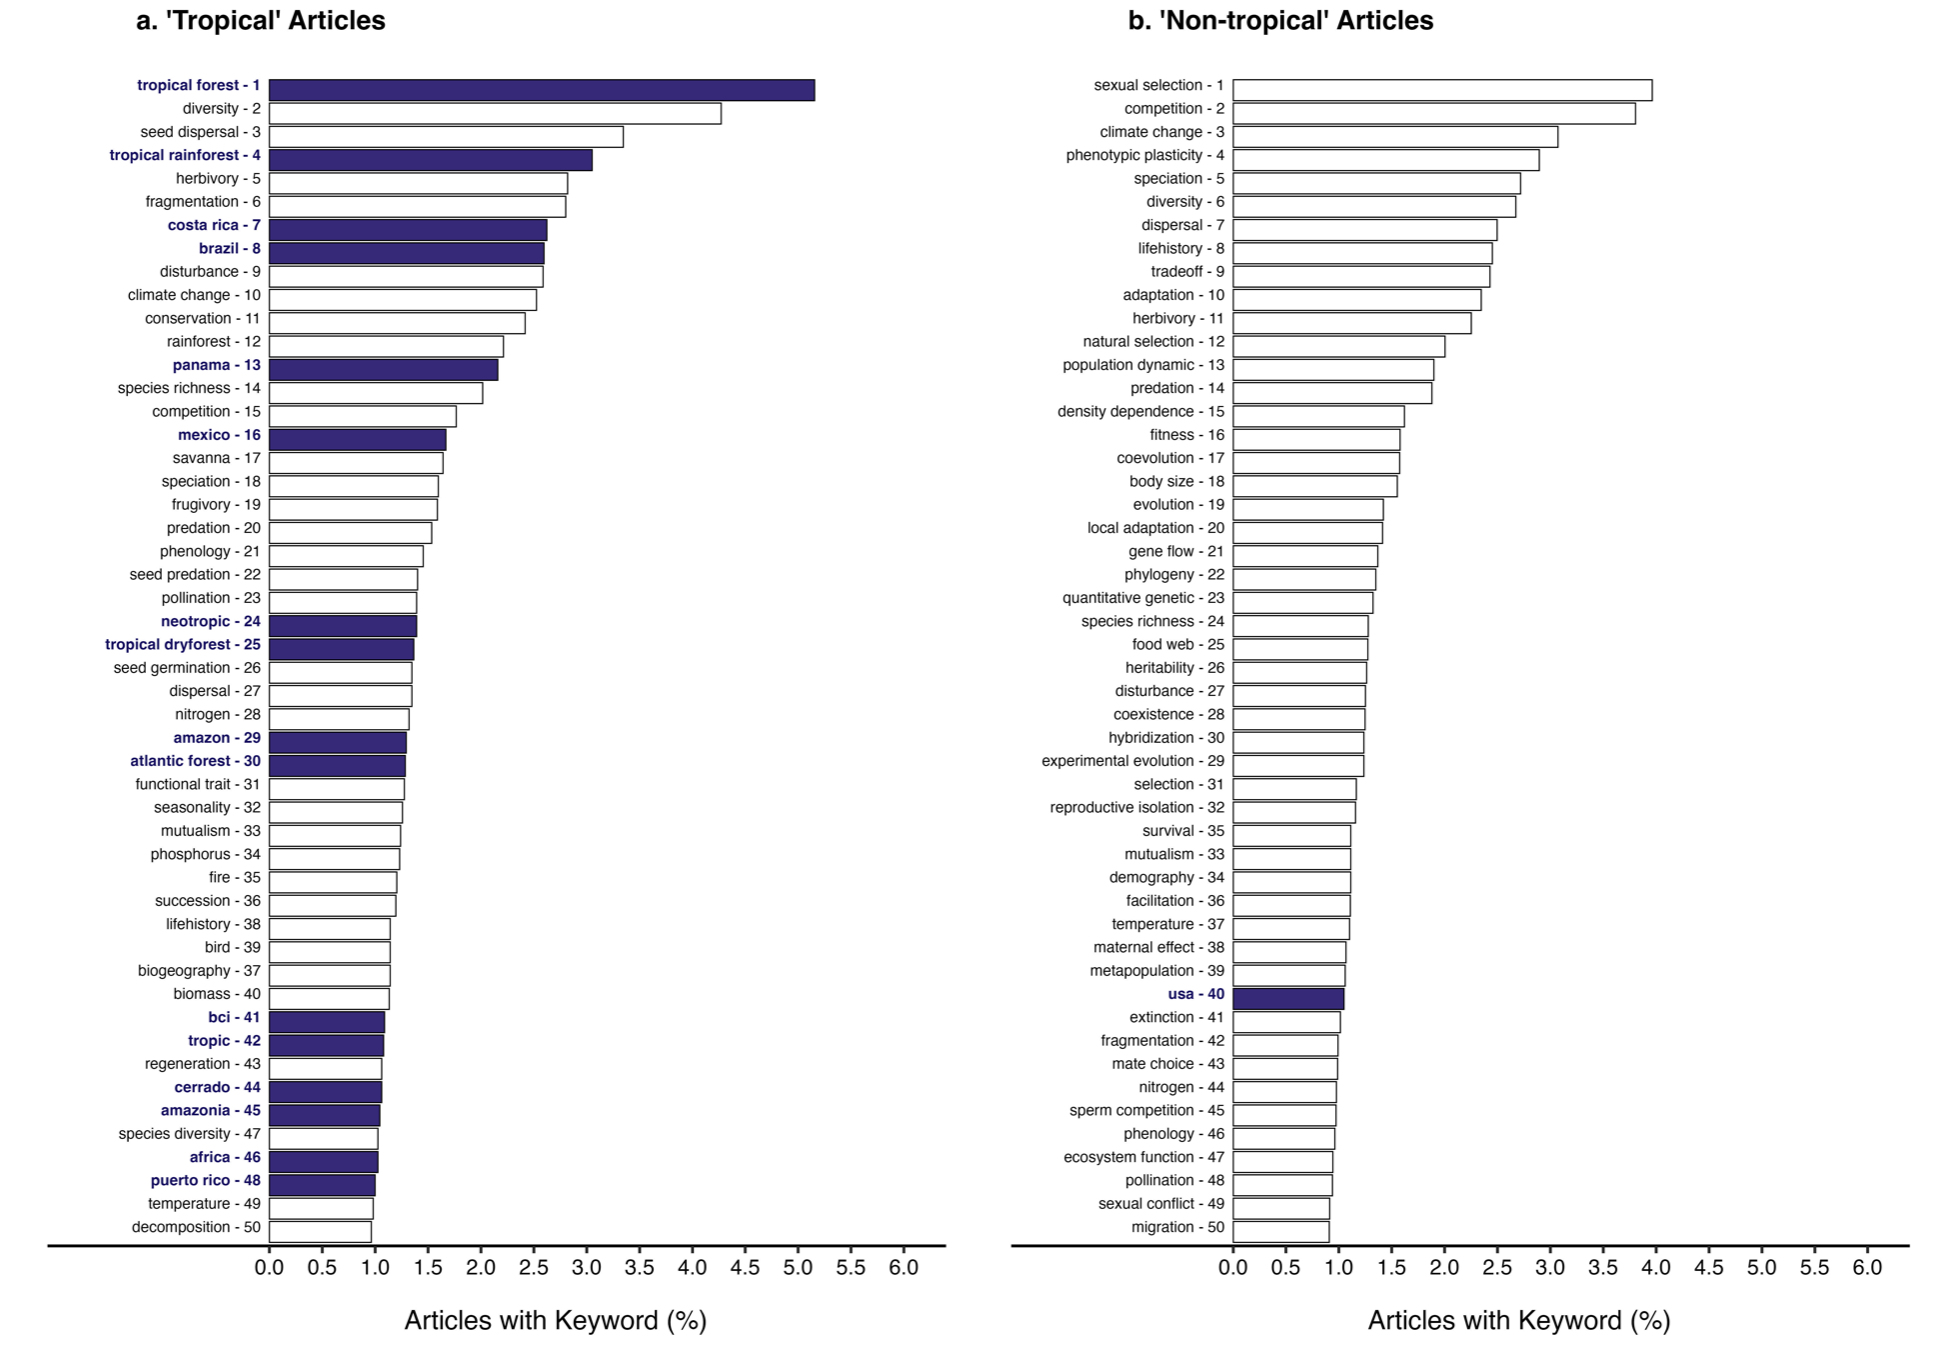
\includegraphics[width=0.9\linewidth,height=0.9\textheight,]{Bruna_plenary_MS_files/figure-latex/keywords-1} 

}

\caption{The N = `r cutoff` most common keywords from articles based on research conducted in (a) the tropics and (b) non-tropical regions. The rank of these words is based on the percentage of articles in each category that included them. Terms reflecting geography (e.g., \textit{tropics, Peru, Southern}) are indicated in bold and with filled bars.}\label{fig:keywords}
\end{figure}

\newpage

\begin{figure}[H]

{\centering 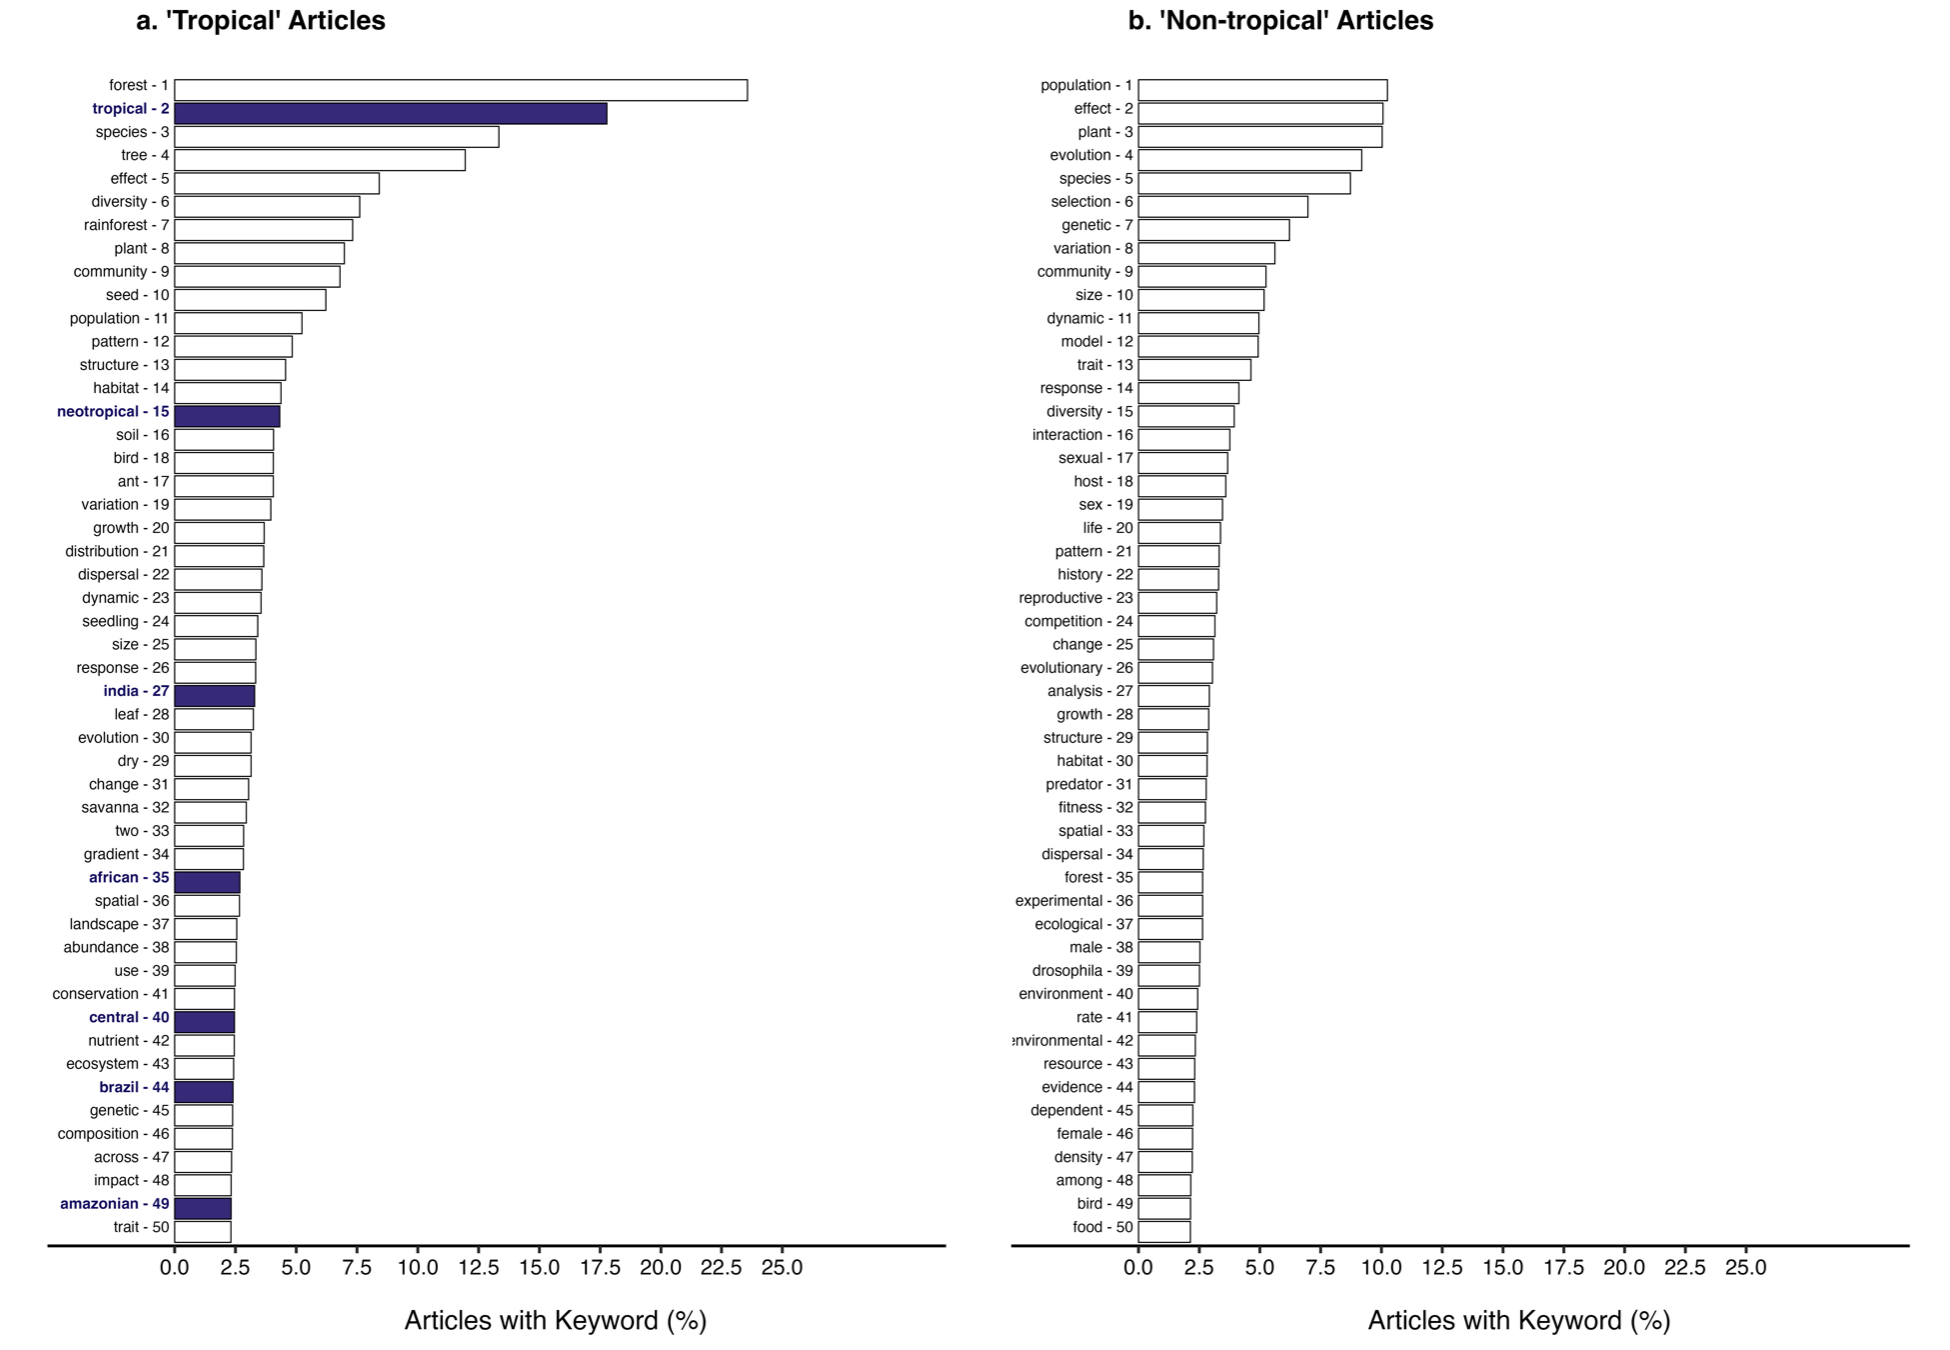
\includegraphics[width=0.9\linewidth,height=0.9\textheight,]{Bruna_plenary_MS_files/figure-latex/titlewords-1} 

}

\caption{The N = `r cutoff` most common words in the titles of articles based on research conducted in (a) the tropics and (b) non-tropical regions. The rank of these words is based on the percentage of article titles in each category that included those words. Terms reflecting geography (e.g., \textit{tropics, Peru, Southern}) are indicated in bold and with filled bars.}\label{fig:titlewords}
\end{figure}

\newpage

\begin{figure}[H]

{\centering 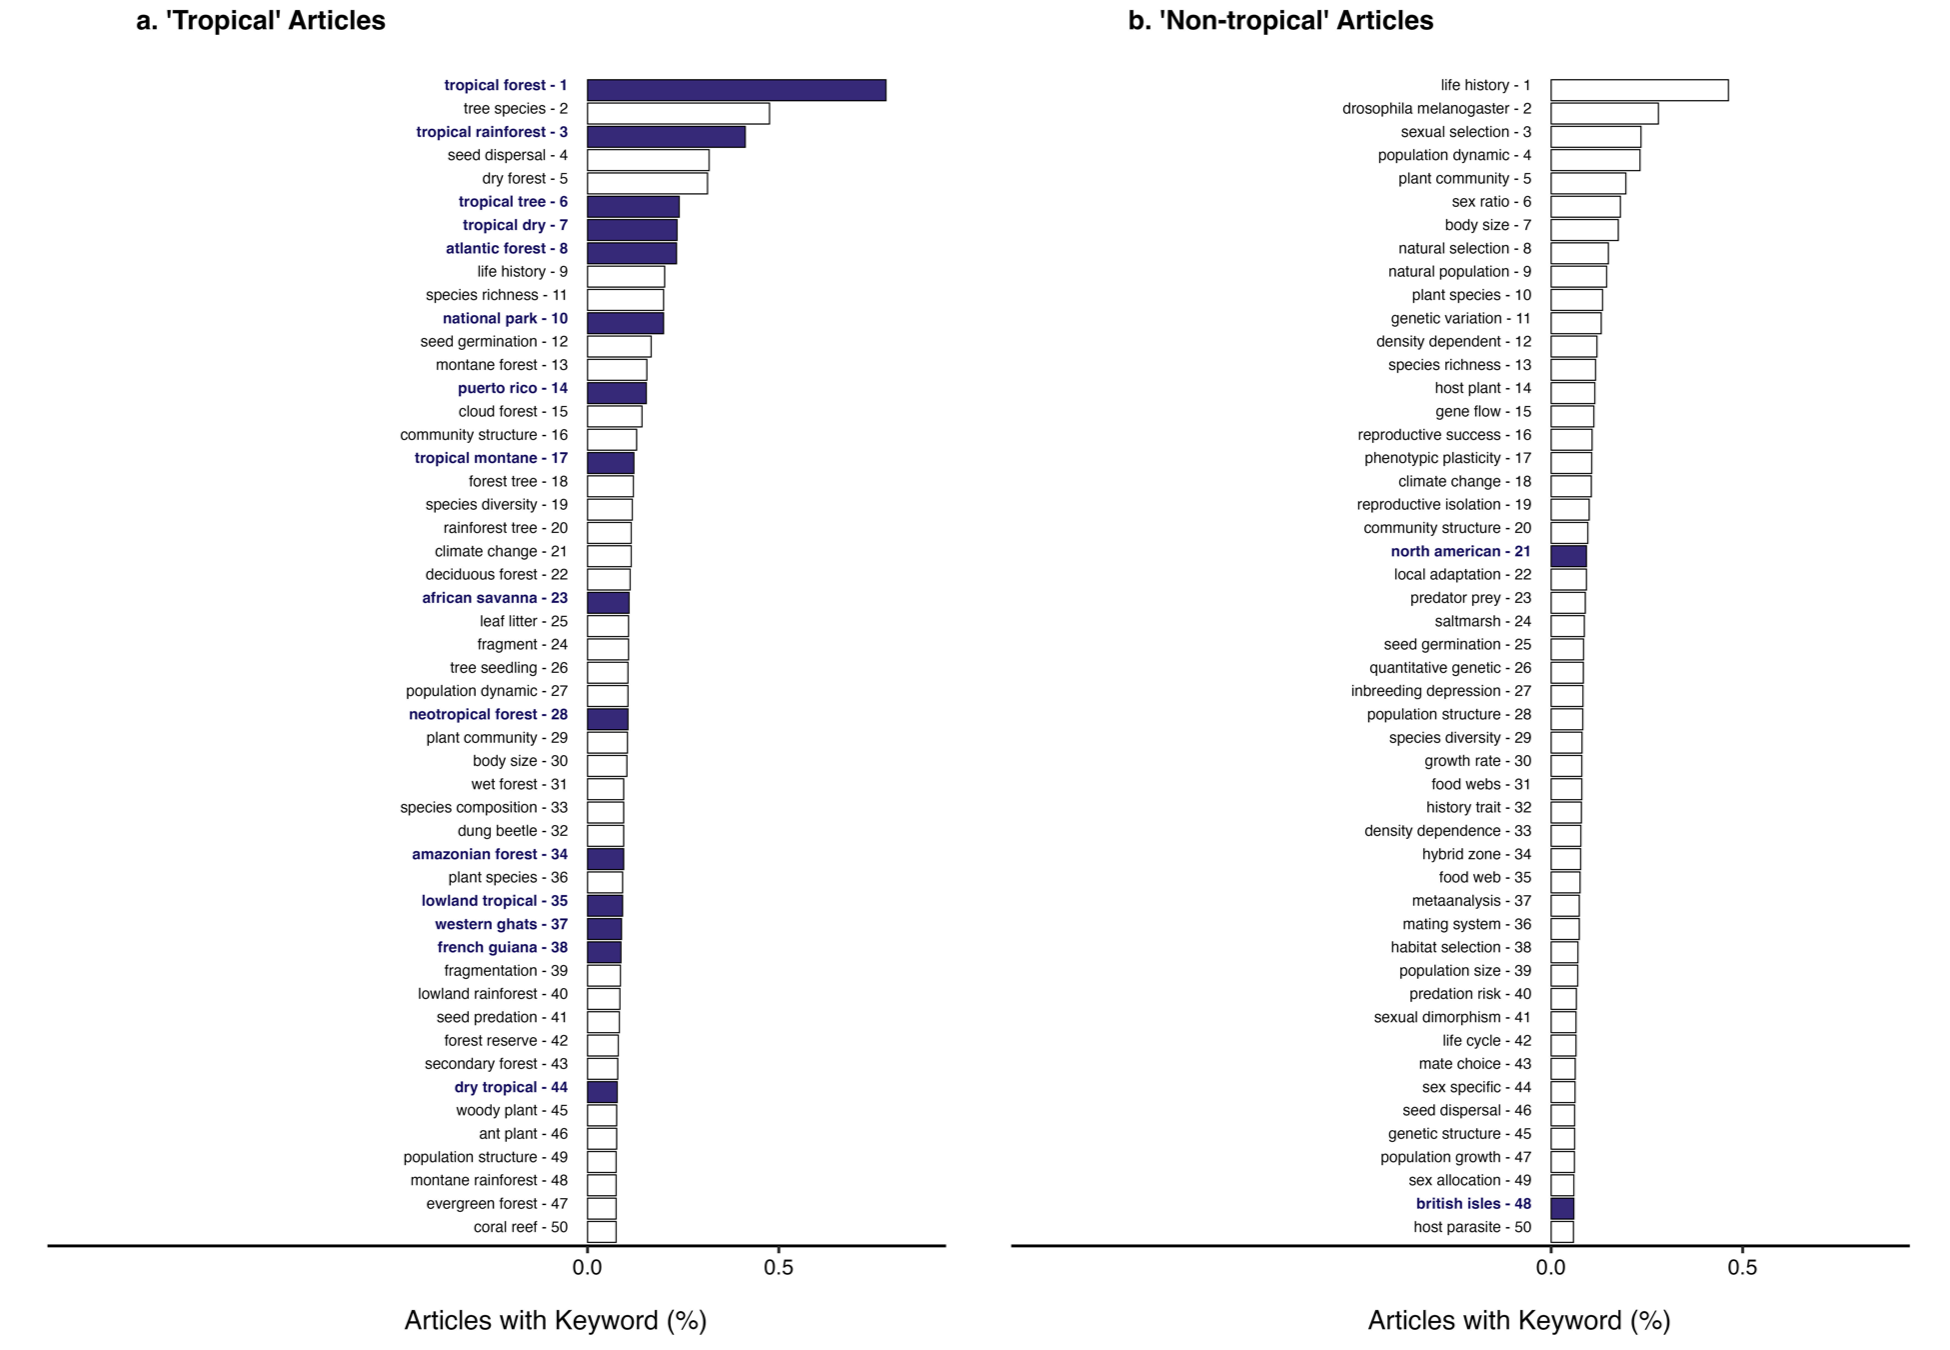
\includegraphics[width=0.9\linewidth,height=0.9\textheight,]{Bruna_plenary_MS_files/figure-latex/bigrams-1} 

}

\caption{The N = `r cutoff` most common bigrams in titles of articles based on research conducted in (a) the tropics and (b) non-tropical regions. The rank of these words is based on the percentage of article titles in each category that included those words. Bigrams reflecting geography (e.g., \textit{tropics, Peru, Atlantic Forest}) are indicated in bold and with filled bars.}\label{fig:bigrams}
\end{figure}

\elandscape
\newpage

\begin{figure}[H]

{\centering 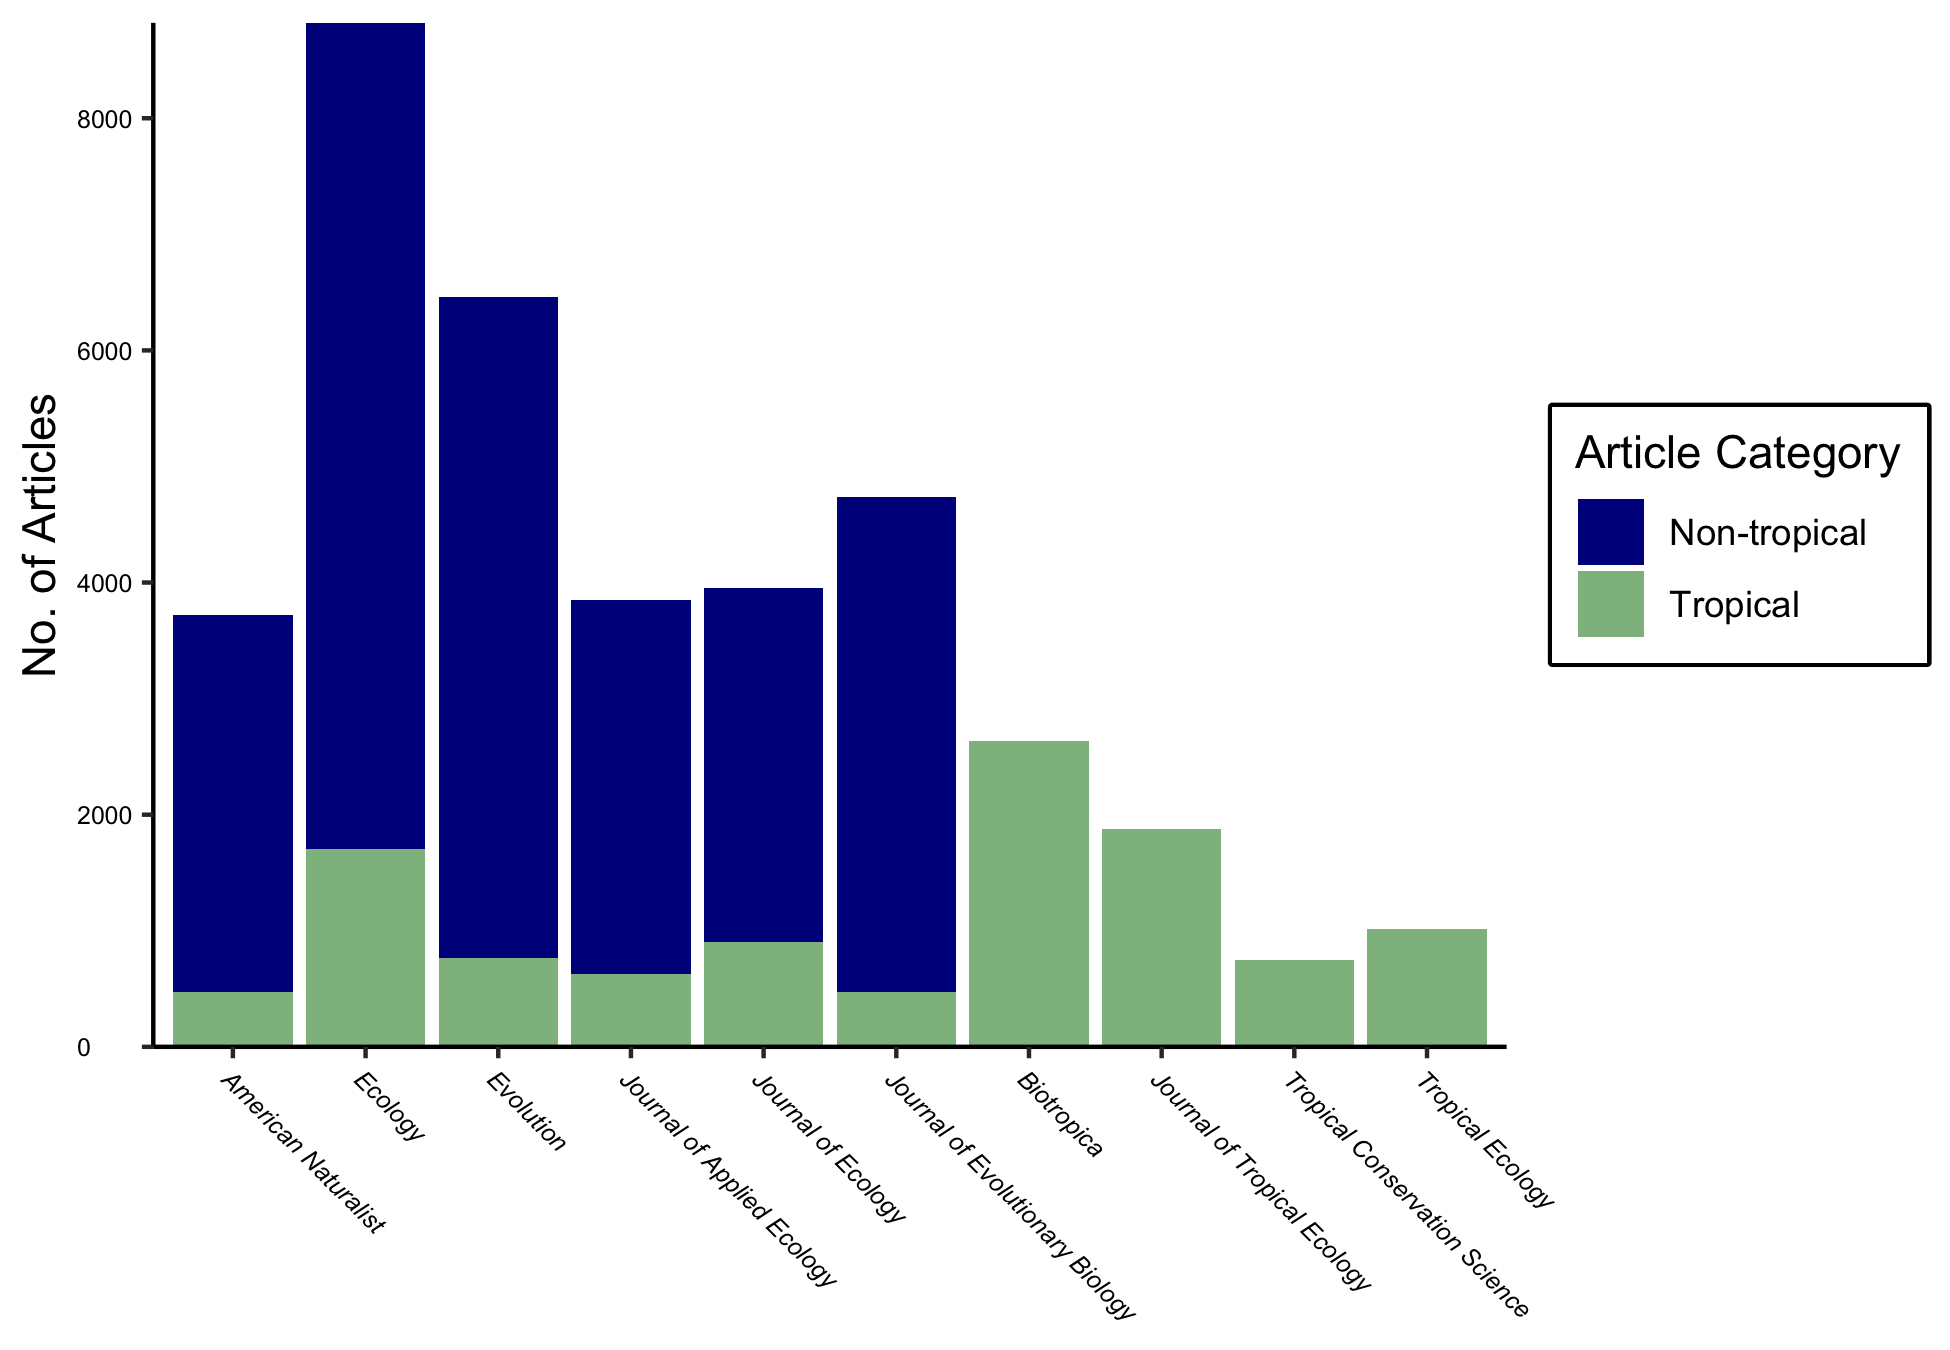
\includegraphics[width=0.9\linewidth,height=0.9\textheight,]{Bruna_plenary_MS_files/figure-latex/kwtime-1} 

}

\caption{The number of articles from each journal and geographic category that were used in used the analysis of keywords.}\label{fig:kwtime}
\end{figure}
\newpage

\begin{figure}[H]

{\centering 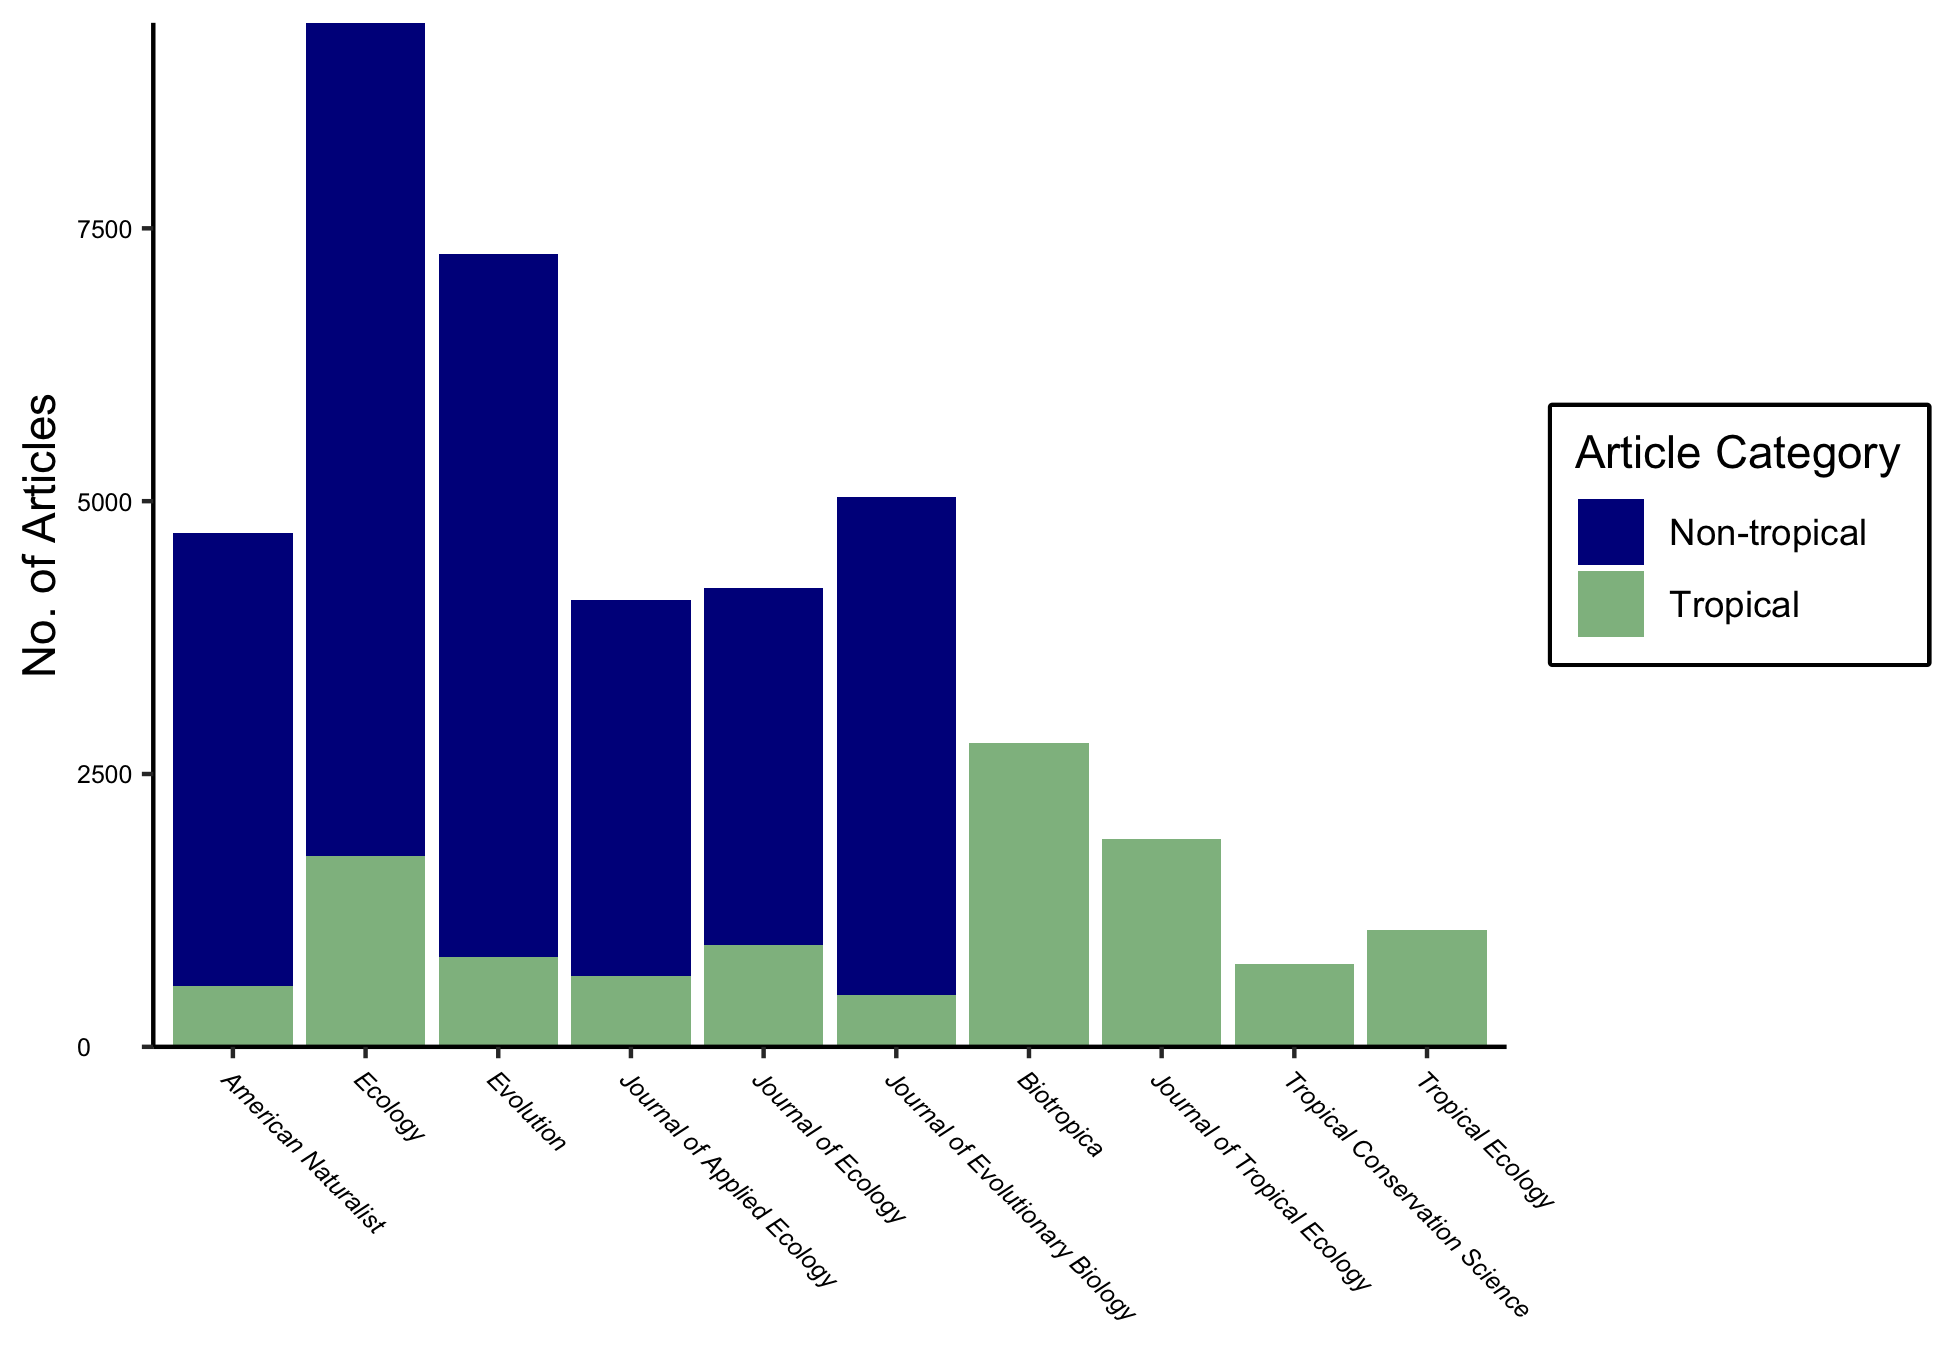
\includegraphics[width=0.9\linewidth,height=0.9\textheight,]{Bruna_plenary_MS_files/figure-latex/twtime-1} 

}

\caption{The number of articles from each journal and geographic category that were used in the analysis of title words and title bigrams.}\label{fig:twtime}
\end{figure}


\end{document}
